\documentclass[twoside]{ctuthesis}

% extra balíky a jejich nastavení

\usepackage{todonotes} % todos
\usepackage{blindtext} % lorem
\usepackage{csquotes}  % quotes
\usepackage{wrapfig}

\usepackage{svg}
\svgpath{img/}

\usepackage[all]{nowidow} % fix for orphaned lines of text
\usepackage{fancyvrb}
\usepackage{siunitx}
\usepackage{sectsty}
\usepackage{titlecaps}
\usepackage{cprotect}
\usepackage{framed}
\usepackage{subcaption}

\usepackage{tabularx}
\usepackage{tabulary}
\usepackage{longtable}
\usepackage{tabu} % longtabu

\usepackage{pmboxdraw}

\usepackage{xcolor}
\definecolor{RubineRed}{HTML}{C30067}

\usepackage{flafter} % ensures embeds won't go before their references
\usepackage{enumitem} % better list spacing

\usepackage{bigfoot} % verbatin in footnote
\usepackage{makecell} % cells with custom align in tabular
\usepackage{tabto} % tabs, but kinda buggy
\usepackage{ragged2e} % this was supposed to improve text alignment

% some symbols. skip integrals because asmmath also defines them and is loaded by the thesis class
\usepackage[nointegrals]{wasysym}

\usepackage[style=numeric,backend=biber,sorting=none]{biblatex}

% Uvozovky v češtině
\iffalse
	% makro pro uvozovky
	\renewcommand\uv[1]{\enquote{#1}}
	% \DeclareQuoteStyle{czech}
	 	{\quotedblbase}
	 	{\textquotedblleft}
	 	{\textquoteleft}
	 	{\textquoteright}
\fi

%% MINTED
\usepackage{minted}    % code listings 
\usepackage{xpatch,letltxmacro}
\LetLtxMacro{\cminted}{\minted}
\let\endcminted\endminted
\xpretocmd{\cminted}{\RecustomVerbatimEnvironment{Verbatim}{BVerbatim}{}}{}{}
\newminted{ini}{frame=leftline,autogobble=true}


%% CTUTHESIS CONFIG

\ctusetup{
	xdoctype = M,
	front-list-of-tables = false,
	mainlanguage = english,
	%
	author = {Ondřej Hruška},
	supervisor = {doc. Ing. Radislav Šmíd, Ph.D.},
	%
	title-english = {Learning and automation GPIO platform},
	title-czech = {Výuková a automatizační GPIO platforma},
	%
	xfaculty = F3,
	department-czech = {Katedra měření},  
	fieldofstudy-czech = {Kybernetika a~robotika},
	subfieldofstudy-czech = {Senzory a~přístrojová technika},
	%
	department-english = {Department of Measurement},
	fieldofstudy-english = {Cybernetics and Robotics},
	subfieldofstudy-english = {Sensors and Instrumentation},
	front-specification = true,
	specification-file = {zadani-zakryto.pdf},
	%specification-file = {zadani-doc.pdf},
	%specification-file = {zadani-doc.pdf},
	%
	keywords-czech = {},
	keywords-english = {},
	%
	day = 0,     % ???
	month = 0,  % ???
	year = 2018, % ???
}

\ctuprocess

\hypersetup{
	pdftitle = {Learning and automation GPIO platform},
	pdfauthor = {Ondřej Hruška}
}

% Extra info na titulní stránce
\addto\ctucaptionsczech{%
	\def\supervisorname{Vedoucí}%
	\def\subfieldofstudyname{Studijní program}%
}

% Abstrakt, poděkování atd
\ctutemplateset{maketitle twocolumn default}{
	\begin{twocolumnfrontmatterpage}
		\ctutemplate{twocolumn.thanks}
		\ctutemplate{twocolumn.declaration}
		\ctutemplate{twocolumn.abstract.in.titlelanguage}
		\ctutemplate{twocolumn.abstract.in.secondlanguage}
		\ctutemplate{twocolumn.tableofcontents}
		\ctutemplate{twocolumn.listoffigures}
	\end{twocolumnfrontmatterpage}
}



%% SPACING

% Booktabs
\setlength{\heavyrulewidth}{0.5mm}
\setlength{\lightrulewidth}{0.25mm}
\setlength{\cmidrulewidth}{0.25mm}

% More space in table cells
\renewcommand{\arraystretch}{1.4}

% Fix overful hbox
\setlength{\emergencystretch}{.5em}

% -- odstavce --
\setlength\parskip{1.5ex plus 1pt minus 1 pt}
%\setlength{\parskip}{1.5ex plus 0.2ex minus 0.1ex} % po změně je potřeba doladit nadpisy
%\renewcommand{\baselinestretch}{1.1}
\setlength\parindent{.5cm}

% add blank page unless current is left
%\newcommand*\cleartoleftpage{%
%	\clearpage
%	\ifodd\value{page}\hbox{}\newpage\fi
%}

% don't clear page before chapter
%\renewcommand{\cleardoublepage}{\clearpage}

% section on new page, except first
%\pretocmd{\section}{%
%	\ifnum\value{section}=0 \else\clearpage\fi
%}{}{}

% ??? what does this do
\makeatletter
\newcommand*{\centerfloat}{%
	\parindent \z@
	\leftskip \z@ \@plus 1fil \@minus \textwidth
	\rightskip\leftskip
	\parfillskip \z@skip}
\makeatother



%% LINK COLORS
\hypersetup{
	colorlinks,
	linkcolor={red!50!black},
	citecolor={blue!50!black},
	urlcolor={blue!80!black}
}


%% HELPER MACROS

\newcommand\nobr[1]{\mbox{#1}}

% monospace
\newcommand\mono[1]{\texttt{#1}}

% library name
\newcommand\lib[1]{\textit{#1}}

% název listing figure
% \renewcommand\listingscaption{Program}

% \newcommand\zdroj[1]{\textit{Zdroj: #1}}


%% UNITS

\newcommand{\uF}{\micro\farad}
\newcommand{\nF}{\nano\farad}
\newcommand{\cm}{\centi\metre}
\newcommand{\VperA}{\V/\A}

\newcommand{\IIC}{I\textsuperscript{2}C\xspace}
\newcommand{\IIS}{I\textsuperscript{2}S\xspace}
\newcommand{\arm}{Arm\xspace}
\newcommand{\armcm}{Arm Cortex-M\xspace}
\newcommand{\mbed}{Arm Mbed\xspace}

\newcommand*\xCmdName[2]{#1~(#2)\xspace}

\newcommand*\CmdSuccess{\xCmdName{0x00}{Success}}
\newcommand*\CmdPing{\xCmdName{0x01}{Ping}}
\newcommand*\CmdError{\xCmdName{0x02}{Error}}
\newcommand*\CmdBulkReadOffer{\xCmdName{0x03}{Bulk~Read~Offer}}
\newcommand*\CmdBulkReadPoll{\xCmdName{0x04}{Bulk~Read~Poll}}
\newcommand*\CmdBulkWriteOffer{\xCmdName{0x05}{Bulk~Write~Offer}}
\newcommand*\CmdBulkData{\xCmdName{0x06}{Bulk~Data}}
\newcommand*\CmdBulkEnd{\xCmdName{0x07}{Bulk~End}}
\newcommand*\CmdBulkAbort{\xCmdName{0x08}{Bulk~Abort}}
\newcommand*\CmdUnitRequest{\xCmdName{0x10}{Unit~Request}}
\newcommand*\CmdUnitReport{\xCmdName{0x11}{Unit~Report}}
\newcommand*\CmdListUnits{\xCmdName{0x20}{List~Units}}
\newcommand*\CmdINIRead{\xCmdName{0x21}{INI~Read}}
\newcommand*\CmdINIWrite{\xCmdName{0x22}{INI~Write}}
\newcommand*\CmdPersistConfig{\xCmdName{0x23}{Persist~Config}}



% a coloured inttype label with \item in the payload table
\newcommand{\cfieldx}[1]{{\color{RubineRed} \texttt{#1}}}
\newcommand{\cfield}[1]{\item \cfieldx{#1}\,} % \tabto{1cm}

\newcommand{\cname}[1]{\textbf{#1}\newline}

% https://tex.stackexchange.com/questions/157389/how-to-center-column-values-in-a-table
% P will be a centered column that can have width
\newcolumntype{P}[1]{>{\centering\arraybackslash}p{#1}}
\newcolumntype{W}[1]{>{\raggedright\arraybackslash}p{#1}}

% this is put before a response that follows a request
% this is needed for nice looking spacing
\newcommand*{\cjoin}{\null\vspace*{-2pt}}

% This is a table of commands of events
\newenvironment{cmdlist}
{
	\tabulinesep=5pt
	\begin{longtabu} to \textwidth {P{2.2em} X[3] X[3,l]}			
		\toprule		
		\textbf{Code} & \textbf{Function} & \textbf{Structure} \\
		\midrule
		\endhead
		
		\bottomrule	
		\endfoot
}{
	\end{longtabu}
}

% a list of generic payload fields
\newenvironment{pldlist}
{
	\begin{itemize}[
		leftmargin=.7cm,
		rightmargin=1mm,
		nosep		
	]
}
{
	\end{itemize}
}


% a list of request fields, with a caption
\newenvironment{cmditemlistenv}[1]
{
	\begin{minipage}[t]{\linewidth}
		
	\begin{flushleft} % fix weird spacing in wrapped lines
	
	\textit{#1} % the caption, like Request: or Response:
	\begin{pldlist}	
}
{
	\end{pldlist}
	\end{flushleft}

	% the minipage somehow fixes vertical alignment 
	% and also removes mysterious spacing around the itemize
	\end{minipage}
}


% a list of request fields, with a caption
\newenvironment{cmdreq}
{
	\begin{cmditemlistenv}{Request:}	
}
{
	\end{cmditemlistenv}	
}

% a list of request fields, with a caption
\newenvironment{cmdresp}
{
	\begin{cmditemlistenv}{Response:}	
}
{
	\end{cmditemlistenv}
}

% a list of payload fields, with a caption
\newenvironment{cmdpld}
{
	\begin{cmditemlistenv}{Payload:}		
}
{
	\end{cmditemlistenv}
}


%% hack from https://tex.stackexchange.com/questions/145812/using-fbox-in-a-newenvironment
% to allow using fbox inside a environment
\newsavebox{\mybox}

% a list of payload fields, with a caption
\newenvironment{boxedpayload}[1][]
{
	\begingroup\setlength{\fboxsep}{0pt}
	\indent
	\begin{lrbox}{\mybox}
	\begin{minipage}{\textwidth - \parindent*2}\null
	\ifthenelse{\equal{#1}{}}{
		\vspace{3pt} % no title
	}{
		% with title
		\hspace{6pt}\textit{#1}
		\vspace{-6pt}\newline
		\noindent\rule{\textwidth}{.4pt}		
		\vspace{-\baselineskip}
		\vspace{-4pt}
	}
	\begin{itemize}[
		itemsep=0pt, % this is not actually 0, for some reason. that's okay
		leftmargin=24pt,
		rightmargin=1mm
	]
}
{
	\end{itemize}
	\vspace{-\baselineskip}
	\vspace{14pt}
	\end{minipage}
	\end{lrbox}\fbox{\usebox{\mybox}}
	\endgroup
}









 % import balíků a nastavení ctuthesis

% --- obsah zvláštních oddílů ---

% Abstrakt

\begin{abstract-english}
This thesis documents the development of a universal software and hardware platform providing high-level user applications running on a PC with access to GPIO pins, hardware buses, and signal acquisition and generation functions, using USB, USART, or a wireless connection.

The requirements of common engineering tasks and problems occurring in the university environment were evaluated to design an extensible, reconfigurable hardware module that would make a versatile and low-cost tool that in some cases eliminates the need for professional measurement and testing equipment.

We designed custom hardware modules, an extensible microcontroller firmware, and PC support libraries for programming languages C and Python. The Python library may further  be used in MATLAB scripts. The devices provide access to hardware buses (\IIC, SPI, USART, and 1-Wire) and microcontroller peripherals (GPIO, ADC, and DAC), implement frequency measurement and other useful features. They are configured in INI files accessed through on a virtual USB mass storage device, or programmatically.
\end{abstract-english}

\begin{abstract-czech}
\begin{otherlanguage}{czech}
Tato práce popisuje vývoj univerzální softwarové a~hardwarové platformy pro přístup k~hardwarovým sběrnicím a~elektrickým obvodům z~prostředí vysokoúrovňových programovacích jazyků a~aplikací běžících na PC, a~to za využití USB, UARTU a~také bezdrátově.

Byly vyhodnoceny požadavky typických problémů vyskytujících se při práci s~vestavěnými systémy a~ve výuce za účelem návrhu snadno rozšiřitelného a~přenastavitleného hardwarového modulu který bude praktickým, pohodlným a~dostupným nástrojem, který navíc v~některých případech může nahradit profesionální laboratorní přístroje.

Bylo navrženo několik prototypů hardwarových modulů spolu s~obslužnými knihovnami v~jazycích C a~Python; Python knihovnu lze dále používat z~prostředí MATLAB. Navržené moduly umožňují přístup k~většině běžných hardwarových sběrnic (\IIC, SPI, USART, 1-Wire) a~umožňují také měřit frekvenci a~vzorkovat či generovat analogové signály.
\end{otherlanguage}
\end{abstract-czech}

% Acknowledgements
\begin{thanks}

\todo[inline]{TODO}

\end{thanks}

% Declaration / Prohlaseni
\begin{declaration}

Prohlašuji, že jsem předloženou práci vypracoval samostatně a~že jsem uvedl veškeré použité informační zdroje v~souladu s~Metodickým pokynem o~dodržování etických principů při přípravě vysokoškolských závěrečných prací.

\medskip

V~Praze, 25. května 2018

\vspace*{.5cm}

...........................................



\end{declaration}


%\addbibresource{thesis.bib}
\bibliography{thesis.bib}
% Buses and peripherals
\newacronym{ADC}{ADC}{Analog/Digital Converter}
\newacronym{DAC}{DAC}{Digital/Analog Converter}
\newacronym{DDS}{DDS}{Direct Digital Synthesis}
\newacronym{SPI}{SPI}{Serial Peripheral Interconnect}
\newacronym{USART}{USART}{Universal Synchronous/Asynchronous Receiver/Transmitter}
\newacronym{UART}{UART}{Universal Asynchronous Receiver/Transmitter}
\newacronym[sort=I2C]{I2C}{I\textsuperscript{2}C}{Inter-Integrated Circuit}
\newacronym[sort=I2S]{I2S}{I\textsuperscript{2}S}{Inter-IC Sound}
\newacronym{USB}{USB}{Universal Serial Bus}
\newacronym{CAN}{CAN}{Controller Area Network}
\newacronym{HART}{HART}{Highway Addressable Remote Transducer}
\newacronym{LIN}{LIN}{Local Interconnect Network}
\newacronym{DALI}{DALI}{Digital Addressable Lighting Interface}
\newacronym{DMA}{DMA}{Direct Memory Access} % ???
\newacronym{mbus}{M-Bus}{Meter Bus}

\newacronym{STEM}{STEM}{Science, Technology, Engineering and Mathematics}
\newacronym{SSH}{SSH}{Secure Shell}
\newacronym{NRZI}{NRZI}{Non Return to Zero Inverted}
\newacronym{MSC}{MSC}{Mass Storage Class}
\newacronym{CDCACM}{CDC/ACM}{Communication Devices Class / Abstract Control Model}
\newacronym{CDC}{CDC}{Communication Devices Class}
\newacronym{ACM}{ACM}{Abstract Control Model}
\newacronym{BOT}{BOT}{Bulk Only Transport}
\newacronym{SCSI}{SCSI}{Small Computer System Interface}
\newacronym{IAD}{IAD}{Interface Association Descriptor}
\newacronym{FAT}{FAT}{File Allocation Table}
\newacronym{FS}{FS}{file system}
\newacronym{IDE}{IDE}{integrated desktop environment}
\newacronym{LFN}{LFN}{Long File Name}
\newacronym{MBR}{MBR}{master boot record}
\newacronym{NVIC}{NVIC}{Nested Vectored Interrupt Controller}
\newacronym{GPS}{GPS}{Global Positioning System}
\newacronym{TWI}{TWI}{Two-Wire Interface}
\newacronym{SMBus}{SMBus}{System Management Bus}
\newacronym{PMBus}{PMBus}{Power Management Bus}

% Common names
\newacronym{RMS}{RMS}{root mean square}
\newacronym{PC}{PC}{personal computer}
\newacronym{PCB}{PCB}{printed circuit board}
\newacronym{TVS}{TVS}{transiet-voltage suppressor}
\newacronym{GPIO}{GPIO}{general purpose input/output}
\newacronym{IC}{IC}{integrated circuit}
\newacronym{PWM}{PWM}{pulse width modulation}
\newacronym{LCD}{LCD}{liquid crystal display}
\newacronym{GUI}{GUI}{graphical user interface}
\newacronym{OS}{OS}{operating system}
\newacronym{API}{API}{application programming interface}
\newacronym{LED}{LED}{light emitting diode}
\newacronym{MCU}{MCU}{microcontroller unit}
\newacronym{RAM}{RAM}{random-access memory}
\newacronym{ROM}{ROM}{read-only memory}

\newacronym{TTL}{TTL}{transistor-transistor logic}
\newacronym{RTS}{RTS}{Ready To Send}
\newacronym{CTS}{CTS}{Clear To Send}
\newacronym{SCK}{SCK}{Serial Clock}
\newacronym{MOSI}{MOSI}{Master Out, Slave In}
\newacronym{MISO}{MISO}{Master In, Slave Out}
\newacronym{NSS}{NSS}{Negated Slave Select}
\newacronym{DE}{DE}{Driver Enable}
\newacronym{CSB}{CSB}{Chip Select Bar}
\newacronym{SS}{SS}{Slave Select}
\newacronym{SDA}{SDA}{Serial Data Line}
\newacronym{SCL}{SCL}{Serial Clock Line}
\newacronym{DTR}{DTR}{Data Terminal Ready}
\newacronym{NDIR}{NDIR}{nondispersive infrared}
\newacronym{NFC}{NFC}{near-field communication}
\newacronym{RTC}{RTC}{real-time clock}
\newacronym{GND}{GND}{ground}
\newacronym{CRC}{CRC}{cyclic redundancy check}

\newacronym{VCO}{VCO}{voltage-controlled oscillator}
\newacronym{TCO}{TCO}{temperature-compensated oscillator}
\newacronym{NCO}{NCO}{numerically controlled oscillator}
\newacronym{DC}{DC}{direct current}
\newacronym{SAR}{SAR}{successive approximation register}
\newacronym{AC}{AC}{alternating current}
\newacronym{TSC}{TSC}{Touch Sensing Controller}

\newacronym{OOK}{OOK}{on-off keying}
\newacronym{FSK}{FSK}{frequency-shift keying}
\newacronym{GFSK}{GFSK}{Gaussian frequency-shift keying}
\newacronym{MSK}{MSK}{minimum-shift keying}
\newacronym{GMSK}{GMSK}{Gaussian minimum-shift keying}
\newacronym{BFSK}{BFSK}{binary frequency-shift keying}
\newacronym{GSM}{GSM}{Global System for Mobile communications}

\glsunset{UART}
\glsunset{CDC}
\glsunset{ACM}


% --- vlastní dokument ---

\begin{document}

\maketitle % titulní strana a automatické oddíly

\part{Introduction}
\chapter{Motivation}

Prototyping, design evaluation, and the measurement of physical properties in experiments make a daily occurrence in the engineering praxis. Those tasks often involve the generation and sampling of electrical signals coming to and from sensors, actuators, and other circuitry.

Recently, a wide range of intelligent sensors became available thanks to the drive to miniaturization in the consumer electronics industry (\cref{fig:some_sensors}). Those devices often provide sufficient accuracy and precision while keeping the circuit complexity and cost low. In contrast to analog sensors, here the signal conditioning and processing circuits are built into the sensor itself, and we access it through a digital connection.

\begin{figure}[H]
	\centering
	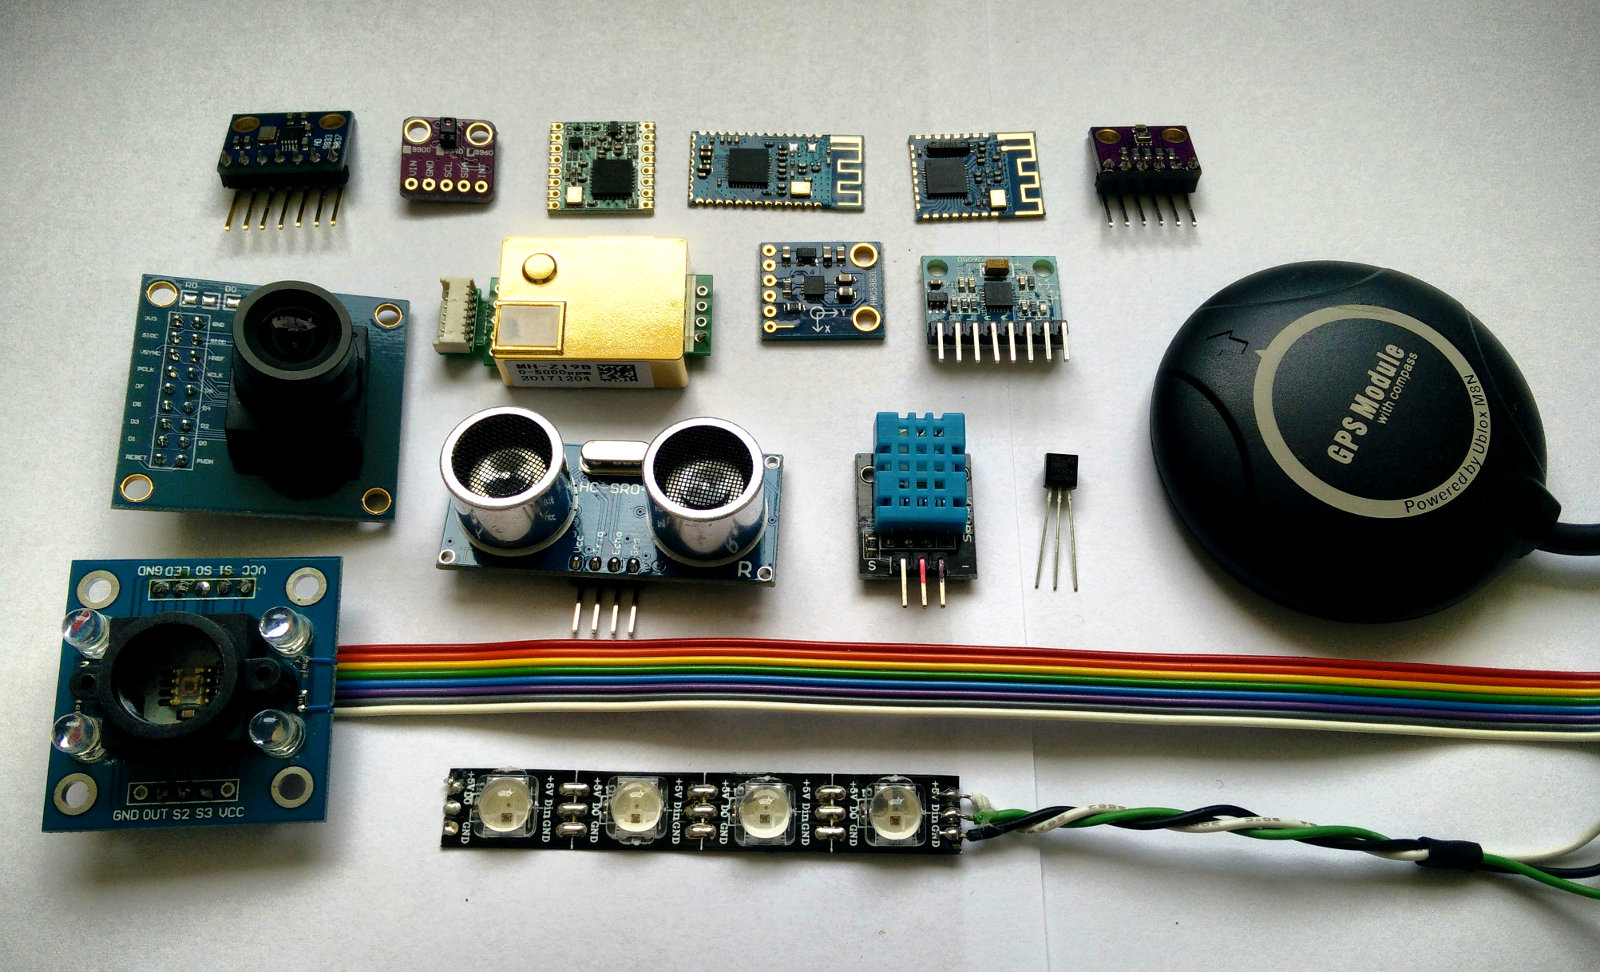
\includegraphics[width=0.8\textwidth] {img/inteligent-sensors.jpg}
	\caption[A collection of intelligent sensors and devices]{\label{fig:some_sensors}A collection of intelligent sensors and devices, most on breadboard adapters: (from the top left) a waveform generator, a gesture detector, a LoRa and two Bluetooth modules, an air quality and pressure sensor, a CO$_2$ sensor, a digital compass, an accelerometer, a GPS module, a camera, an ultrasonic range finder, a humidity sensor, a 1-Wire thermometer, a color detector, and an RGB LED strip}
\end{figure}

If we wish to conduct experiments with these integrated modules, or just familiarize ourselves with a device before using it in a project, we need an easy way to interact with them. It would also be convenient to have direct access to low-level hardware, be it analog signal sampling, generation, or even just the access to logic inputs and outputs. However, advances in computer technology, namely the advent of the \gls{USB}, lead to the disappearance of low-level computer ports, such as the printer port (LPT), that would provide an easy way of doing so.

Today, when we want to perform measurements using a digital sensor, the usual route is to implement embedded firmware for a microcontroller that connects to the \gls{PC} through \gls{USB}, or perhaps shows the results on a display. This approach has its advantages, but is time-consuming and requires specific knowledge unrelated to the measurements we wish to perform. It would be advantageous to have a way to access hardware without having to burden ourselves with the technicalities of this connection, even at the cost of lower performance compared to specialized devices or professional tools.

The design and implementation of such a universal instrument is the object of this work. For technical reasons, such as naming the source code repositories, we need a name for the project; it shall be hereafter called \textbf{GEX}, a name derived from ``\textbf{G}PIO \textbf{Ex}pander''.

\section{Expected Outcome}\label{sec:expected_outcome}

It has been a long-time desire of the author to create a universal instrument connecting low-level hardware to a computer, and, with this project, it is finally being realized. Several related projects approaching this problem from different angles can be found on the internet; some of these will be presented in \cref{sec:prior_art}. 

Our project is not meant to end as a tinkering tool that will be produced in a few prototypes and then forgotten. By creating an extensible, open-source platform, GEX can become the foundation for future projects which others can expand, re-use, and adapt to their specific needs.

\iffalse
\begin{figure}[H]
	\centering
	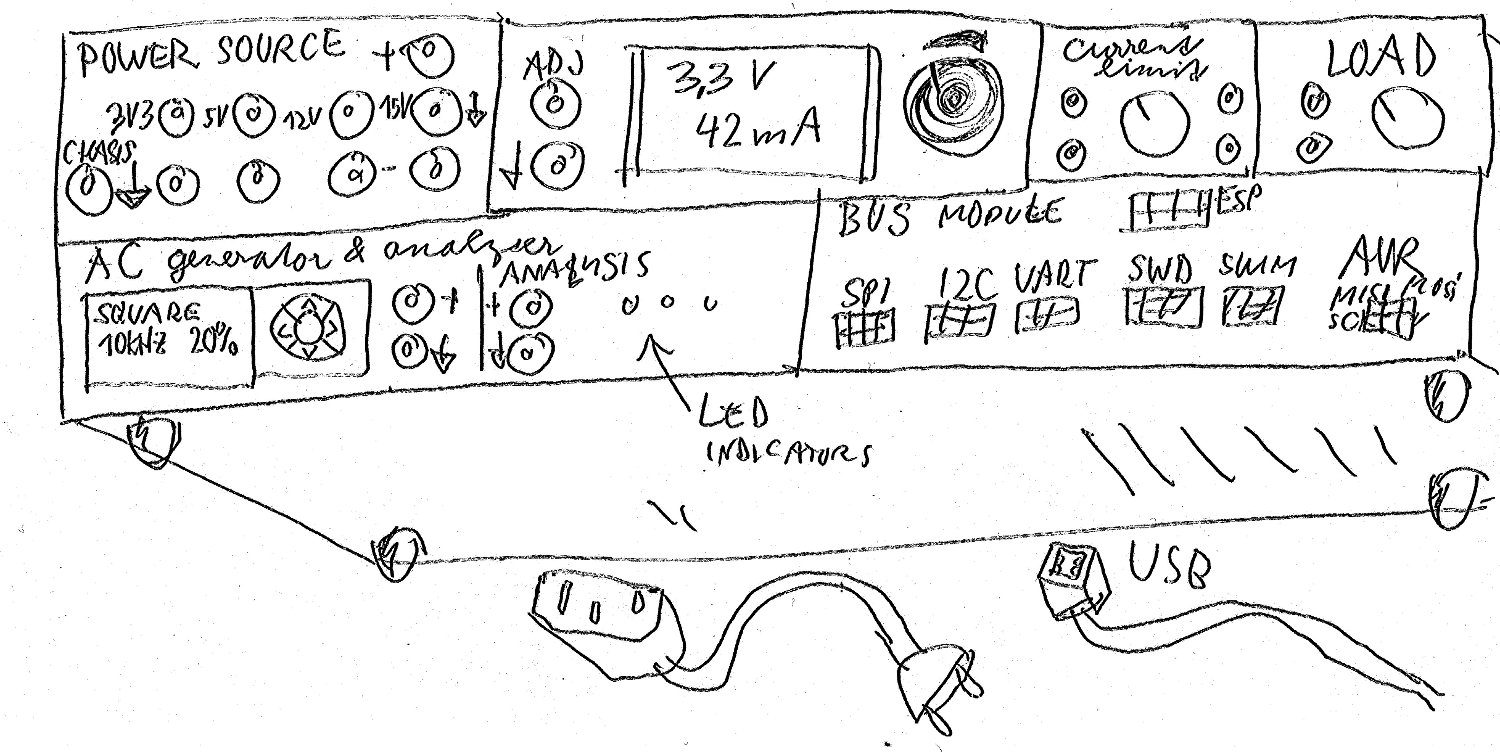
\includegraphics[width=0.7\textwidth] {img/early-sketch.jpg}
	\caption[An early sketch of a universal bench device]{An early (2016) sketch of a universal bench device including a power supply, electronic load, a signal generator and a bus module. The bottom half of the panel is in a large part implemented by GEX.}
\end{figure}
\fi

Building on the experience with earlier embedded projects, an STM32 microcontroller will be used. Those are \armcm devices with a wide range of hardware peripherals that should be a good fit for the project. Low-cost evaluation boards are available that could be used as a hardware platform instead of developing a custom \gls{PCB}. STM32 microcontrollers are affordable and already popular in the embedded hardware community, so there is a real possibility of the project gathering a community around it and growing beyond what will be presented in this paper.

\iffalse
Besides the use of existing development boards, custom \glspl{PCB} will be developed in different form factors. The possibilities of wireless connection should be evaluated. This feature should make GEX useful for instance in mobile robotics or when installed in poorly accessible locations.
\fi








\chapter{Requirement Analysis}

We'll now investigate some situations where GEX could be used, to establish its requirements and desired features.

\section{Desired Features}

\subsection{Interfacing Intelligent Modules}\label{sec:uses-digital-ifaces}

When adding a new digital sensor or a module to a hardware project, we want to test it first, learn how to properly communicate with it and confirm its performance. Based on this evaluation we decide whether the module matches our expectations and learn how to properly connect it, which is needed for a successful \gls{PCB} layout.

In experimental setups, this may be the only thing we need. Data can readily be collected after just connecting the module to a \gls{PC}, same as commanding motor controllers or other intelligent devices.

A couple well known hardware buses have established themselves as the standard ways to interface digital sensors and modules: \gls{SPI}, \gls{I2C} and \gls{USART} (\gls{UART} in asynchronous mode) are the most used ones, often accompanied by a few extra \gls{GPIO} lines for features such as Reset, Chip Enable, Interrupt. There are exceptions where silicon vendors have developed proprietary communication protocols that are still used, either for historical reasons or because of their specific advantages. An example is the 1-Wire protocol used by digital thermometers.

Moving to industrial and automotive environments, we can encounter various fieldbuses, Ethernet, \gls{CAN}, current loop, \gls{HART}, \gls{LIN}, \gls{DALI}, RS485 (e.g. for Modbus), \gls{mbus}, PLC-BUS and others. Those typically use transceiver \glspl{IC} and other circuitry, such as \glspl{TVS}, discrete filters, galvanic isolation. They could be supported using add-on boards and additional firmware modules handling the protocol. For simplicity and to meet time constraints, the development of those boards and modules will be left for future expansions of the project.

\subsection{Analog Signal Acquisition}

Sometimes it is necessary to use a traditional analog sensor, capture a transient waveform or to just measure a voltage. GEX was meant to focus on digital interfaces, however giving it this capability makes it much more versatile. Nearly all microcontrollers include an \gls{ADC} which we can use to measure input voltages and, paired with a timer, to records signals varying in time.

Certain tasks, such as capturing transient effects on a thermocouple when inserted into a flame (an example from developing fire-proof materials) demand level triggering similar to that of oscilloscopes. The converter continuously measures the input voltage and a timed capture starts only after a set threshold is exceeded. This can be accompanied by a pre-trigger feature where the timed capture is continuously running and the last sample is always compared with the threshold, recording a portion of the historic records together with the following samples.

\subsection{Analog Signal Output}

An analog signal can not only be measured, but it is often necessary to also generate it. This could serve as an excitation signal for an experiment, for instance to measure the characteristic curves of a diode or a transistor. Conveniently, we can at the same time use GEX's analog input to record the output.

Generating an analog signal is possible using a \gls{PWM} or by a dedicated digital-analog converter included in many microcontrollers. Higher frequencies or resolution can be achieved with a dedicated external \gls{IC}.

\subsection{Logic Level Input and Output}

We've covered some more advanced features, but skipped the simplest feature: a direct access to \gls{GPIO} pins. Considering the latencies of \gls{USB} and the \gls{PC}'s operating system, this cannot be used reliably for ``bit banging'', however we can still accomplish a lot with just changing logic levels - e.g. to control character \glspl{LCD}, or emulate some interfaces that include a clock line, like \gls{SPI}. As mentioned in~\ref{sec:uses-digital-ifaces}, many digital sensors and modules use plain \glspl{GPIO} in addition to the communication bus for out-of-band signaling or features like chip selection or reset.

\subsection{Pulse Generation and Measurement}

Some sensors have a variable frequency or a \gls{PWM} output. To capture those signals and convert them to a more useful digital value, we can use the external input functions of a timer/counter in the microcontroller. Those timers have many possible configurations and can also be used for pulse counting or a pulse train generation.

\section{Host Computer Connection}

\subsection{Communication Interface}

\gls{USB} shall be the primary way of connecting the module to a host \gls{PC}. Thanks to \gls{USB}'s flexibility, it can present itself as any kind of device or even multiple devices at once.

The most straightforward method of interfacing the board is by passing binary messages in a fashion similar to \gls{UART}. We'll need a duplex connection to enable command confirmations, query-type commands and asynchronous event reporting. This is possible either using a ``Virtual COM port'' driver, or through a raw access to the corresponding \gls{USB} endpoints. Using a raw access avoids potential problems with the operating system's driver interfering or not recognizing the device correctly; on the other hand, having GEX appear as a serial port makes it easier to integrate into existing platforms that have a good serial port support (such as National Instruments LabWindows CVI or MATLAB).

A connection using a hardware \gls{UART} is also planned, as a fallback for boards without an USB connector or for platforms with no \gls{USB} connectivity. A wireless connection to the host PC should also be possible and work transparently in a similar way to the \gls{USB} or \gls{UART} connection.

\subsection{Configuration Files}

The module must be easily reconfigurable. Given the settings are almost always going to be tied on the connected external hardware, it would be practical to have an option to store them permanently in the microcontroller's non-volatile memory.

We can load those settings into GEX using the serial interface, which also makes it possible to reconfigure it remotely when the wireless connection is used. With USB, we can additionally make the board appear as a mass storage device and expose the configuration as text files. This approach, inspired by ARM mbed's mechanism for flashing firmware images to development kits, avoids the need to create a configuration \gls{GUI}, instead using the built-in applications of the \gls{PC} \gls{OS}, like file explorer and notepad. We can expose additional information, such as a README file with instructions or a pin-out reference, as separate files on the virtual disk.

\section{An Overview of Planned Features}

Let's now summarize the features we wish to support in the GEX firmware, based on the preceding discussion:

\begin{itemize}
	\item \textbf{Hardware interfacing functions}
		\begin{itemize}
			\item I/O pin direct access (read, write), pin change interrupt
			\item Analog input: voltage measurement, sampled capture
			\item Analog output: static level, waveform generation
			\item Frequency, duty cycle, pulse length measurement
			\item Single pulse and \gls{PWM} generation
			\item \gls{SPI}, \gls{I2C}, \gls{UART}/\gls{USART}
			\item Dallas 1-Wire
			\item NeoPixel (addressable \gls{LED} strips)
		\end{itemize}
	\pagebreak[0]
	\item \textbf{Communication with the host computer}
		\begin{itemize}
			\item \gls{USB} connection as virtual serial port or direct endpoint access
			\item Connection using plain \gls{UART}
			\item Wireless attachment
		\end{itemize}
	\item \textbf{Configuration}
		\begin{itemize}
			\item Fully reconfigurable, temporarily or permanently
			\item Settings stored in INI files
			\item File access through the communication \gls{API} or using a virtual mass storage
		\end{itemize}
\end{itemize}

\section{Microcontroller Selection}

As discussed in section~\ref{sec:expected-outcome}, this project will be based on microcontrollers from the STM32 family. The STM32F072 model was selected for the initial hardware and firmware design due to its low cost, advanced peripherals, and the availability of development boards. The firmware can be ported to other \glspl{MCU} later (e.g. to STM32L072, STM32F103 or STM32F303).

The STM32F072 is a Cortex M0 device with 128\,KiB of flash memory, 16\,KiB of \gls{RAM} and running at 48\,MHz. It is equipped with a \gls{USB} Full Speed peripheral block, a 12-bit \gls{ADC} and \gls{DAC}, a number of general-purpose timers/counters, SPI, I$^2$C, and USART peripherals, among others. It supports crystal-less \gls{USB}, using the USB SOF packet for synchronization of the internal 48\,MHz RC oscillator; naturally, a real crystal resonator will provide better timing accuracy.

To effectively utilize the time available for this work, only the STM32F072 firmware will be developed while making sure the planned expansion is as straightforward as possible.

\section{Form Factor Considerations}

While the GEX firmware can be used with existing evaluation boards from ST Microelectronics (see figure~\ref{fig:discovery} for an example of one such board), we wish to design and realize a few custom hardware prototypes that will be smaller and more convenient to use.

Three possible form factors are drawn in figure~\ref{fig:ff-sketches}. The use of a common connector layout and pin assignments, here Arduino and Raspberry Pi, makes it possible to reuse add-on boards from those platforms. When we copy the physical form factor of another product, in this example the Raspberry Pi Zero, we can further take advantage of existing enclosures designed for it.

\begin{figure}[h]
	\centering
	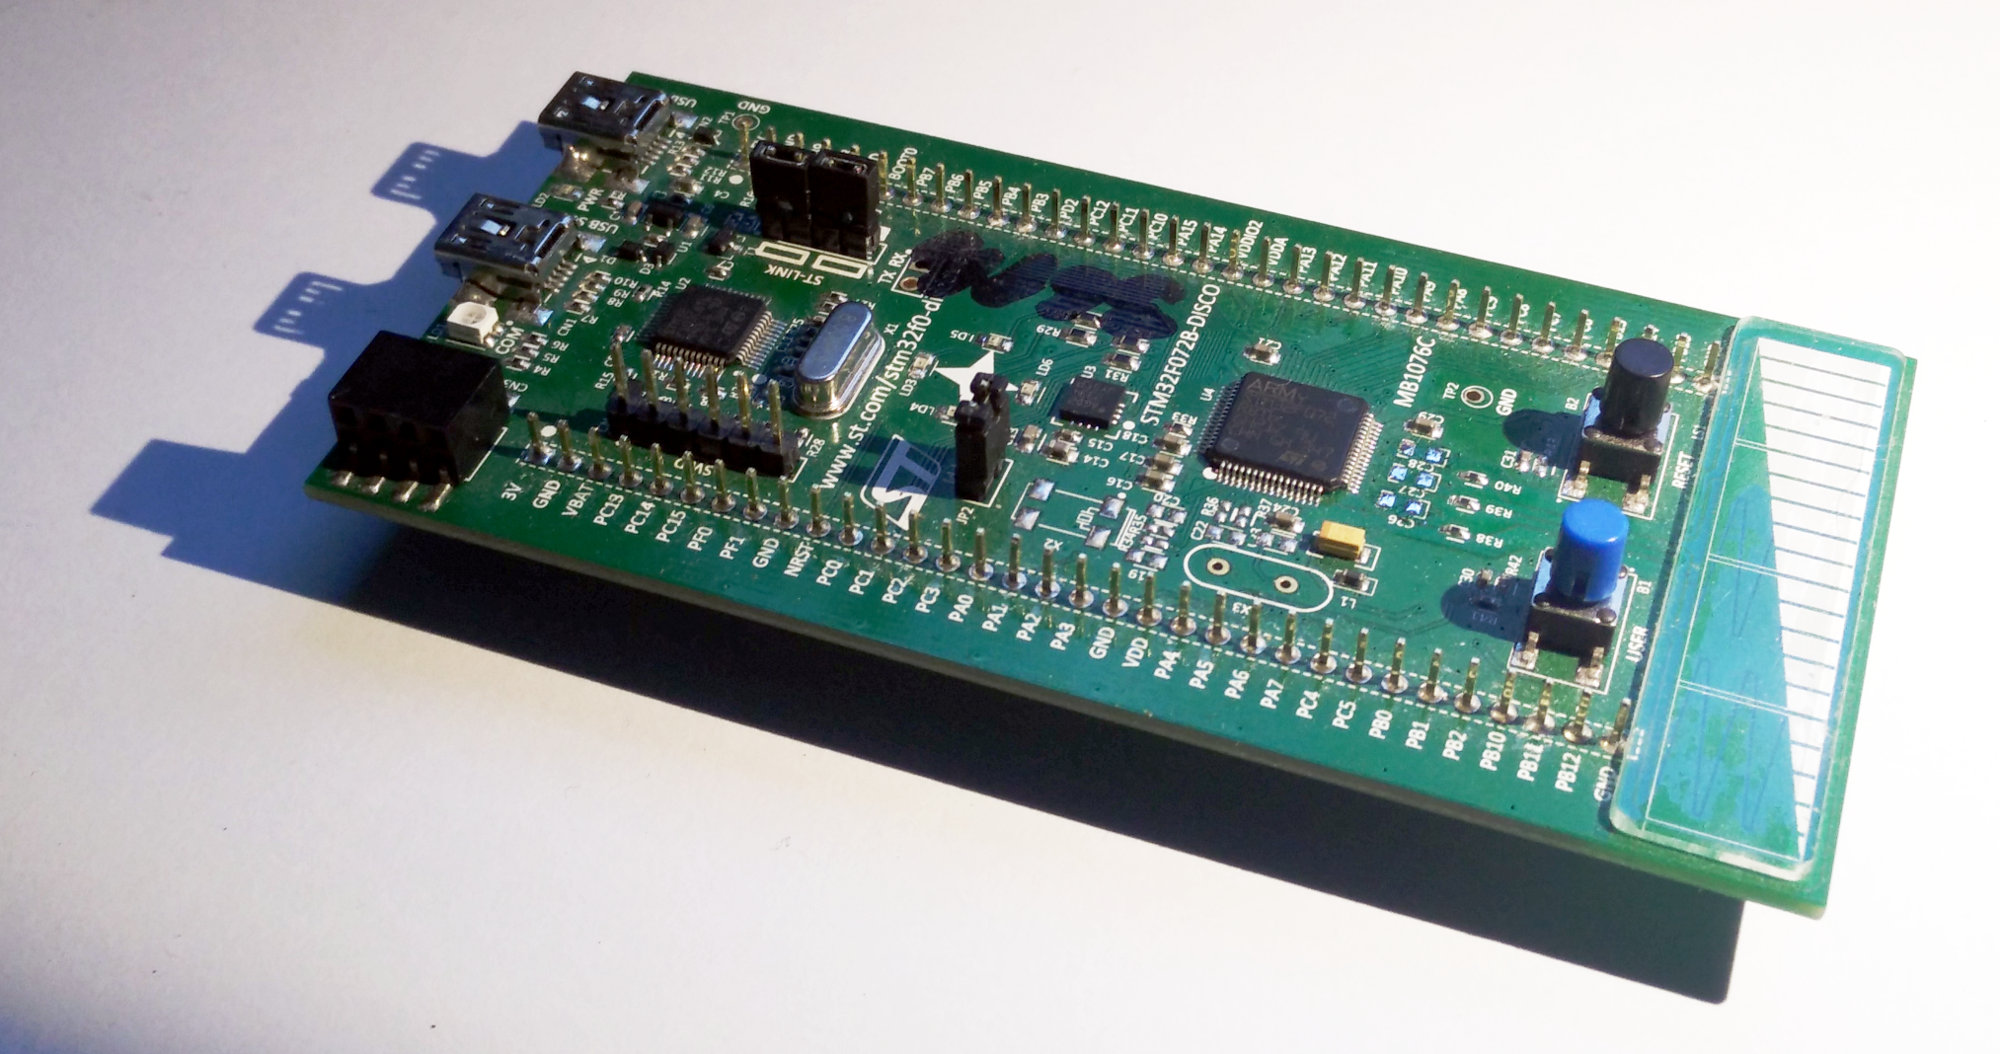
\includegraphics[width=0.7\textwidth] {img/disco072.jpg}
	\caption[A Discovery board with STM32F072]{\label{fig:discovery}A Discovery development board with the STM32F072 microcontroller}
\end{figure}

\begin{figure}[h]
	\centering
	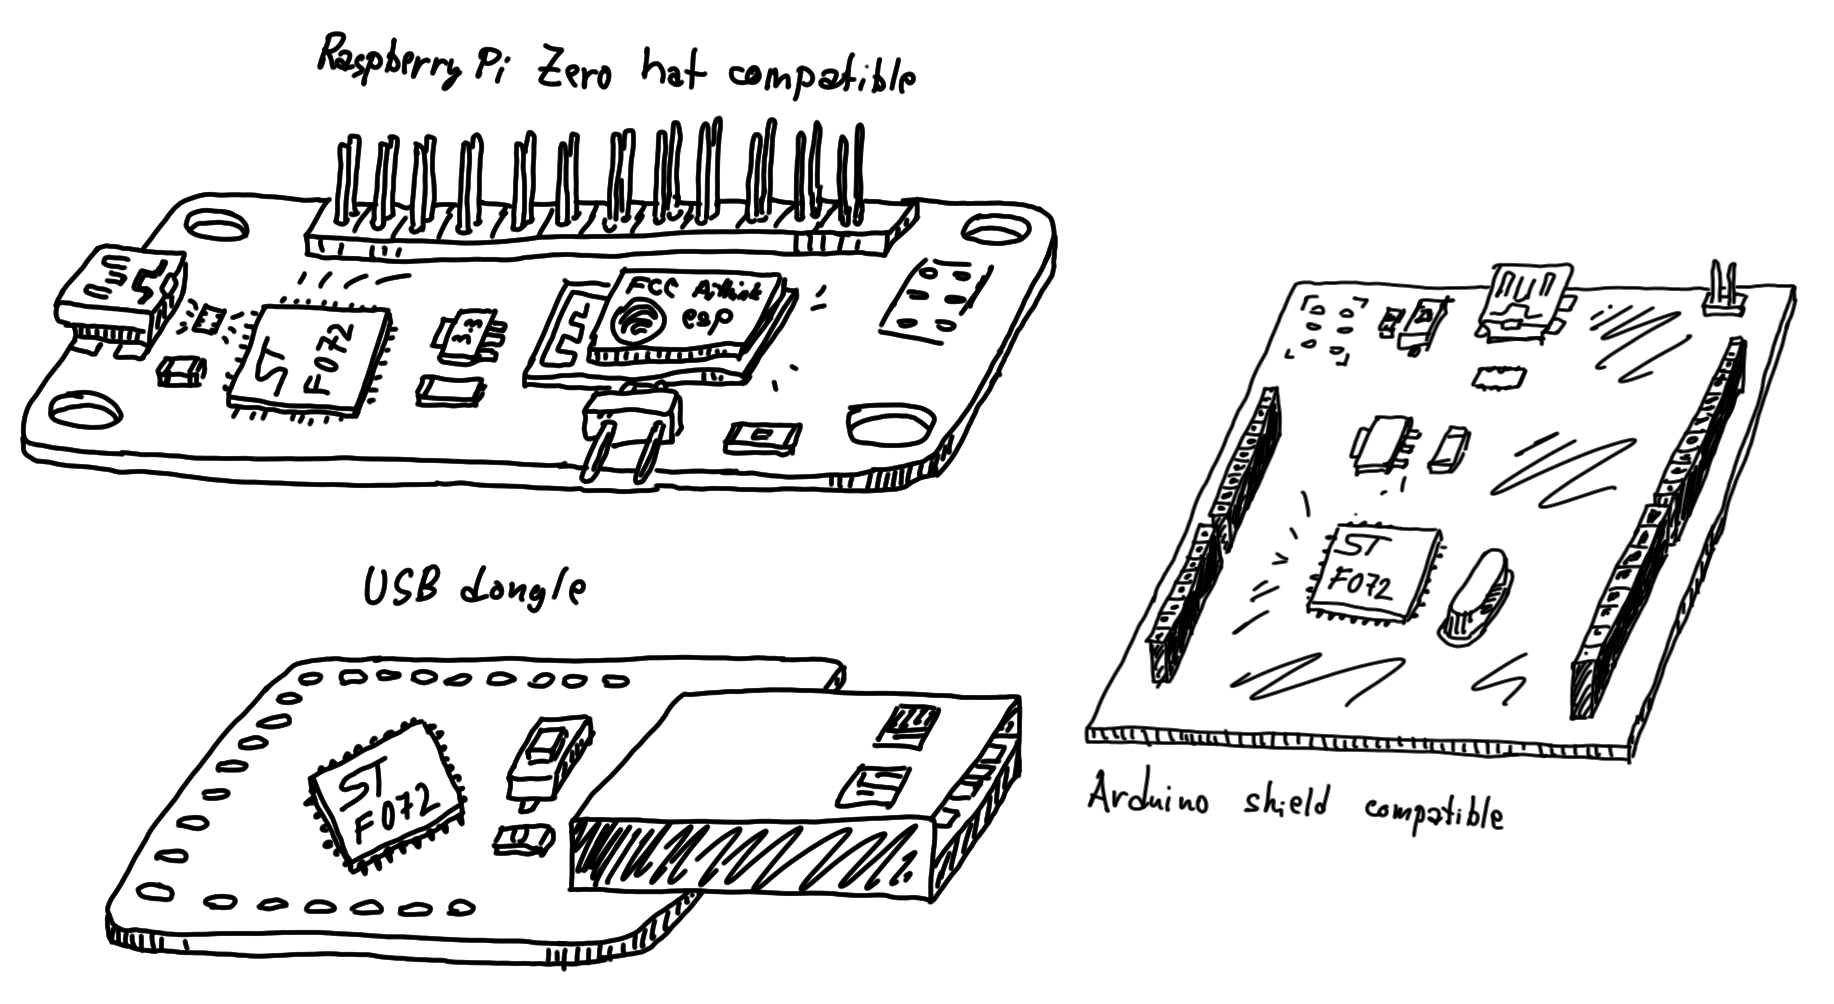
\includegraphics[width=\textwidth] {img/gex-ff-sketches.png}
	\caption[Form factor sketches]{\label{fig:ff-sketches}A sketch of three possible form factors for a GEX hardware realization}
\end{figure}










\chapter{\label{sec:prior-art}Existing Solutions}

The idea of making it easier to interact with low level hardware from a PC is not new. Several solutions to this problem have been developed, each with its own advantages and drawbacks. Some examples will be presented in this chapter.

\section{Bus Pirate}

\begin{figure}[H]
	\centering
	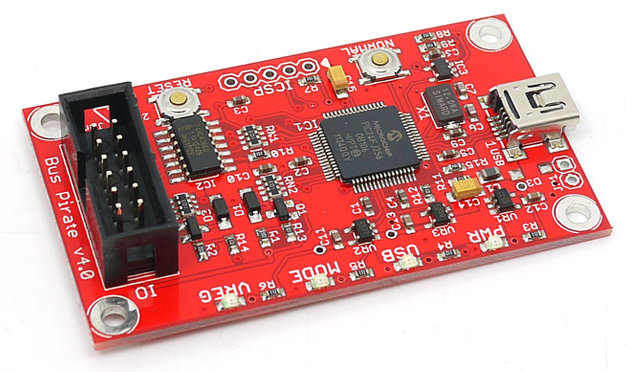
\includegraphics[width=0.6\textwidth] {img/buspirate.jpg}
	\caption{\label{fig:buspirate}Bus Pirate v.4 (picture by \textit{Seeed Studio})}
\end{figure}

\todo[inline]{link to pic source page}

%http://dangerousprototypes.com/blog/about/

Bus Pirate, developed by \todo{link}Ian Lesnet at Dangerous Prototypes and manufactured by Seeed Studio\todo{link}, is a USB-attached device providing access to hardware interfaces like SPI, I$^2$C, USART and 1-Wire, as well as frequency measurement and direct pin access.

The board aims to make it easy for users to familiarize themselves with new chips and modules; it also provides a range of programming interfaces for flashing microcontroller firmwares and memories. It communicates with the PC using a FTDI USB-serial bridge.

Bus Pirate is open source and in scope it's similar to GEX. It can be scripted and controlled from languages like Python or Perl, connects to USB and provides a good selection of hardware interfaces.

The board is based on a PIC16 microcontroller running at 32\,MHz. Its analog/digital converter (ADC) only has a resolution of 10 bits (1024 levels). There is no digital/analog converter (DAC) available on the chip, making applications that require a varied output voltage more difficult. Another limitation of the board is its low number of GPIO pins which may be insufficient for certain applications. The Bus Pirate, at the time of writing, can be purchased for a price similar to some Raspberry Pi models.

\section{Raspberry Pi}

\begin{figure}[H]
	\centering
	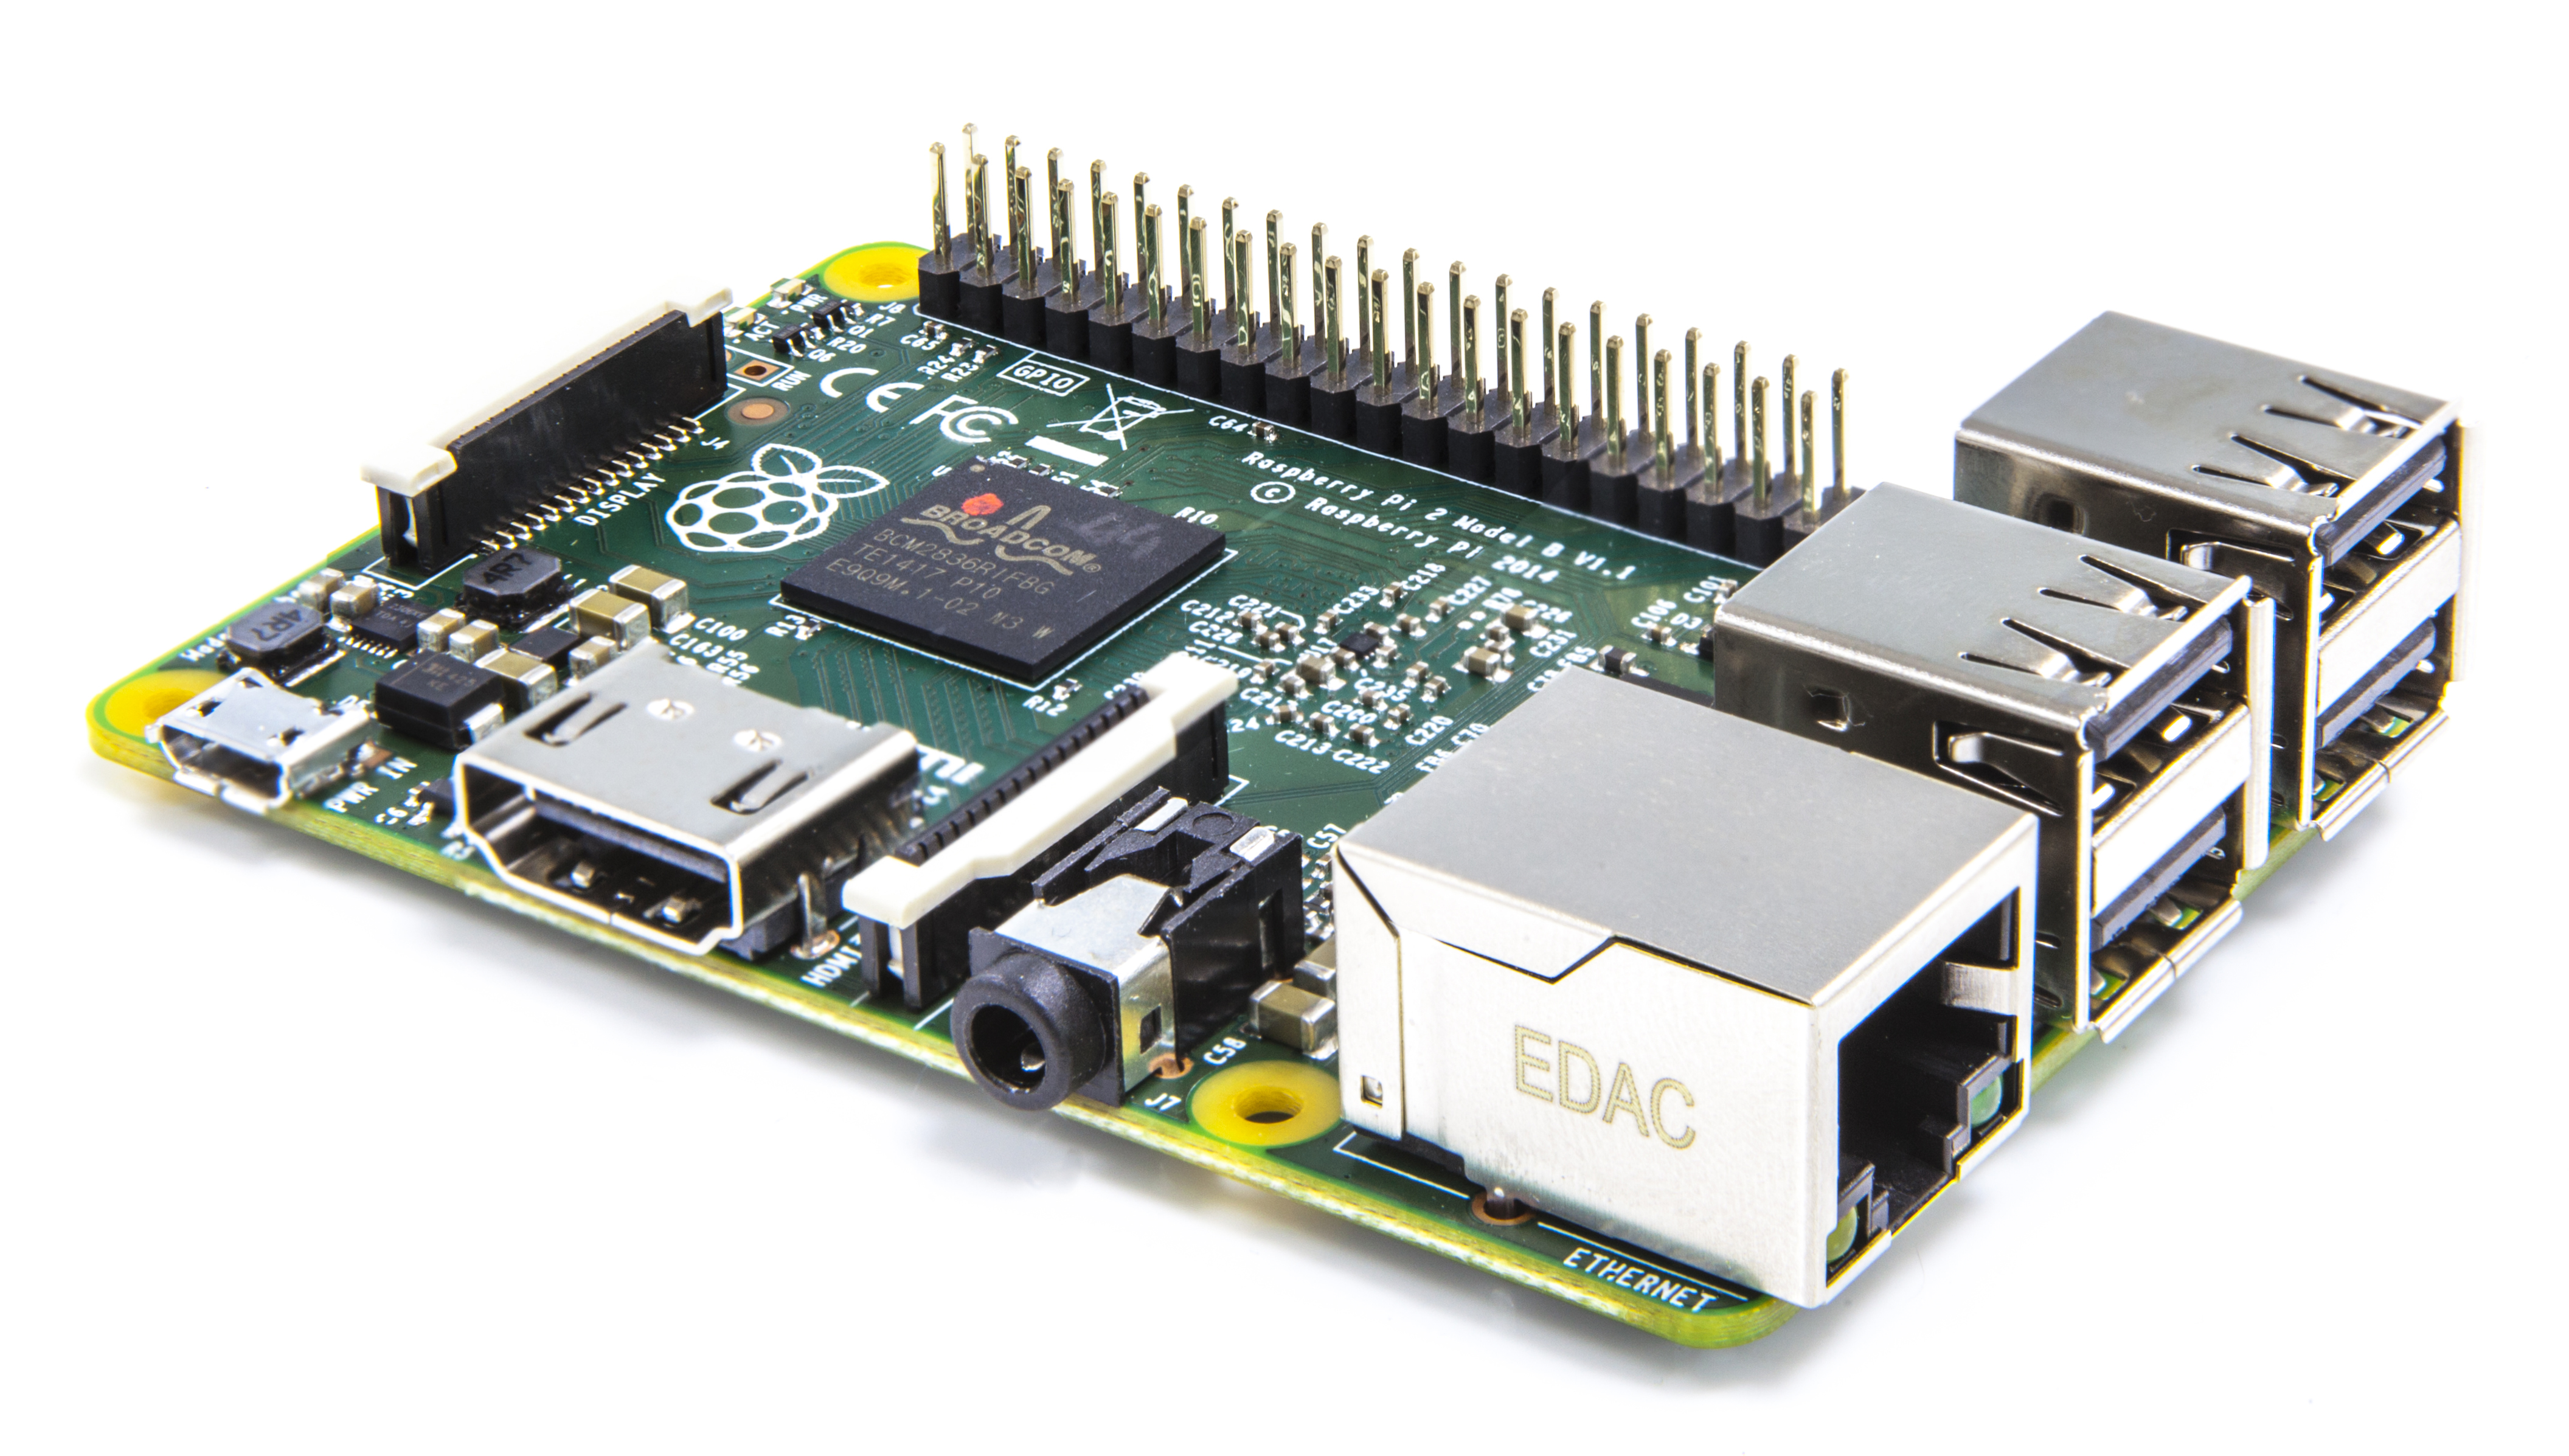
\includegraphics[width=0.6\textwidth] {img/rpi2.jpg}
	\caption{\label{fig:rpi2}Raspberry Pi 2 (picture by \textit{Raspberry Pi Foundation})}
\end{figure}

The Raspberry Pi's GPIO header, which can be directly controlled by user applications, was one of the primary inspirations behind GEX. It can be controlled using C and Python (among others) and offers general purpose I\O, SPI, I2C, UART and PWM, with other protocols being easy to emulate thanks to the high speed of the system processor.

The Raspberry Pi is commonly used in schools as a low-cost PC alternative that encourage students' interest in electronics, programming and science. The board is often built into more permanent projects that make use of its powerful processor, such as wildlife camera traps or home automation projects.

The Raspberry Pi could be used for the same quick evaluations or experiments we want to perform with GEX, however they would either have to be performed directly on the mini-computer itself with attached monitor and keyboard, or use some form of remote access (e.g. SSH). When we have a more powerful computer available, a USB device like GEX would be more convenient.

\section{Professional DAQ Modules}

Various professional tools that would fulfill our needs exist on the market, but their high price makes them inaccessible for users with a limited budget, such as hobbyists or students who would like to keep such a device for personal use. An example is the National Instruments (NI) "I²C/SPI Interface Device" which also includes several GPIO lines, the NI USB DAQ module, or some of the Total Phase I²C/SPI gadgets (figure \ref{fig:profidaq}). The performance GEX can provide may not always match that of those professional tools, but in many cases it'll be a sufficient substitute at a fraction of the cost.

\begin{figure}
	\centering
	\begin{subfigure}{.5\textwidth}
		\centering
		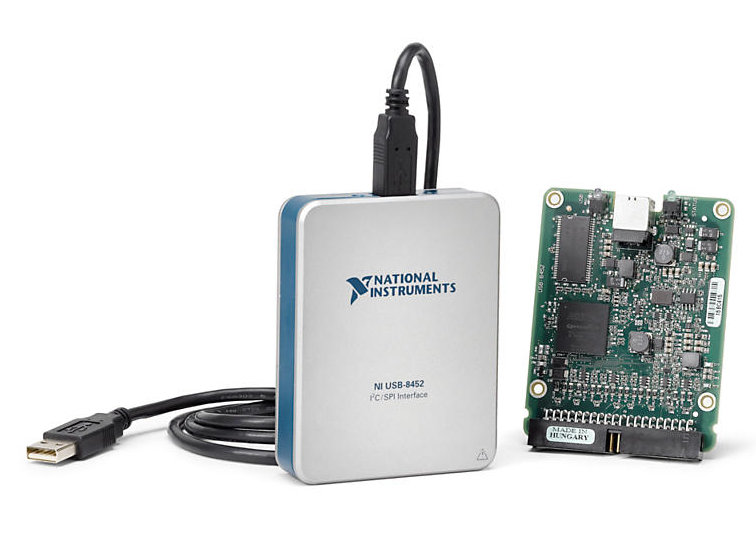
\includegraphics[width=.8\linewidth]{img/ni-i2c-device.jpg}
		\caption{NI I²C/SPI Interface Device}
	\end{subfigure}%
	\begin{subfigure}{.5\textwidth}
		\centering
		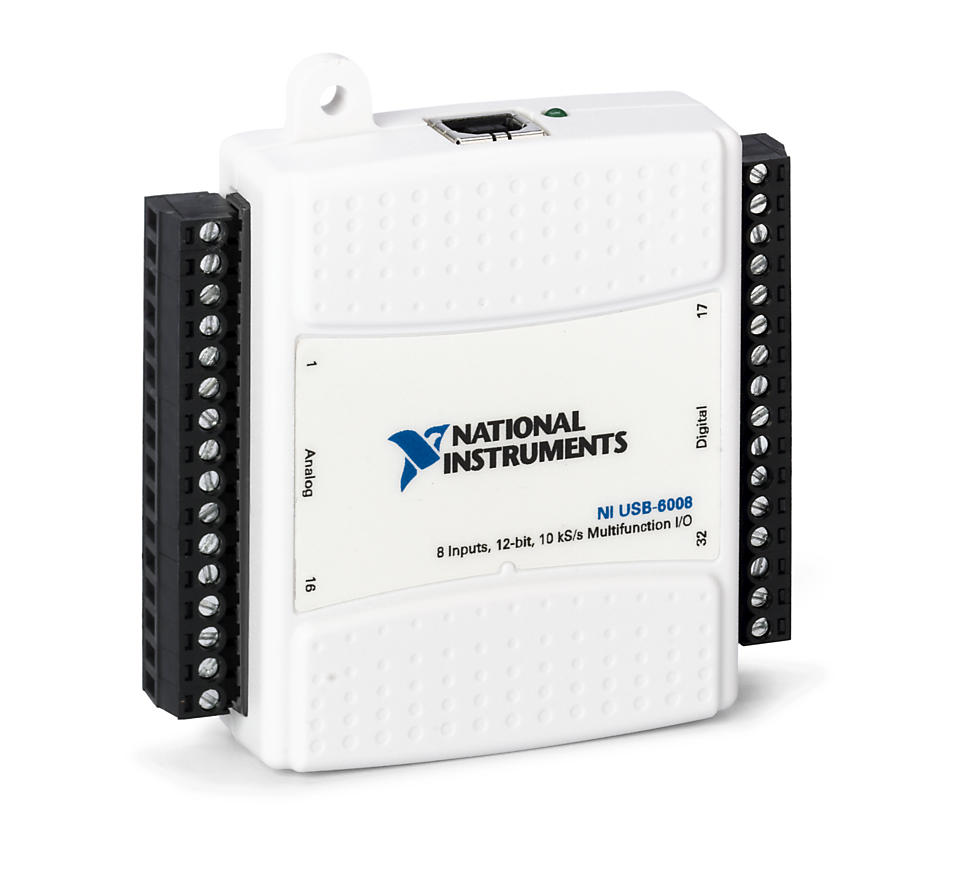
\includegraphics[width=.8\linewidth]{img/nidaq.jpg}
		\caption{NI USB DAQ module}
	\end{subfigure}
	\begin{subfigure}{.5\textwidth}
		\centering
		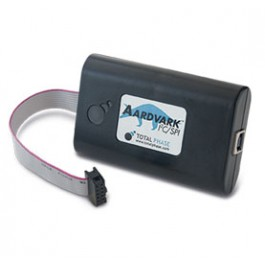
\includegraphics[width=.8\linewidth]{img/total-phase-spi-i2c.jpg}
		\caption{Total Phase SPI/I²C Host "Aardwark"}
	\end{subfigure}
	\caption[Professional tools that GEX can replace]{\label{fig:profidaq}An example of professional tools that GEX could replace in less demanding scenarios (pictures taken from marketing materials)}
\end{figure}

%http://www.ni.com/en-gb/shop/select/i2c-spi-interface-device}

\section{The Firmata Protocol}

\todo[inline]{links}

Firmata is a communication protocol based on MIDI (\textit{Musical Instrument Digital Interface}) for passing data to and from embedded microcontrollers. MIDI is mainly used for attaching electronic musical instruments, such as synthesizers, keyboards, mixers etc., to each other or to a PC. Firmata was designed for Arduino as a high level abstraction for its connection to the PC, typically using a FTDI chip or equivalent.

Implementing Firmata in the GEX firmware would make it possible to use existing Firmata libraries on the PC side. However, the protocol is limited by the encompassing MIDI format and isn't very flexible. 



\part{Theoretical Background}

\chapter{Universal Serial Bus}

This chapter presents an overview of the \acrfull{USB} Full Speed interface, with focus on the features used in the GEX firmware. \gls{USB} is a versatile and powerful interface which replaces several older technologies; for this reason its specification is very complex and going into all details is hardly possible. We will cover the basic principles and terminology of \gls{USB} and focus on the parts relevant for the GEX project. More information about the bus can be found in the official specification \cite{usbif-spec}, related documents published by the USB Implementers Forum, and other on-line resources \cite{usb-nutshell,usb-made-simple}.

\section{Basic Principles and Terminology}

\begin{figure}[h]
	\centering
	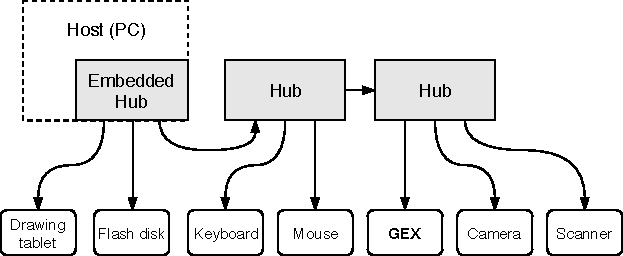
\includegraphics[scale=1] {img/usb-hierarchy-redraw.pdf}
	\caption[USB hierarchical structure]{\label{fig:usb-hierarchy}The hierarchical structure of the USB bus}
\end{figure}

\gls{USB} is a hierarchical bus with a single master (\textit{host}) and multiple slave devices. A \gls{USB} device that provides functionality to the host is called a \textit{function} \cite{usb-function}. 

\subsection{Pipes and Endpoints}

Communication between the host and a function is organized into virtual channels called \textit{pipes} connecting to the device's \textit{endpoints}, identified by endpoint numbers.

\begin{figure}[h]
	\centering
	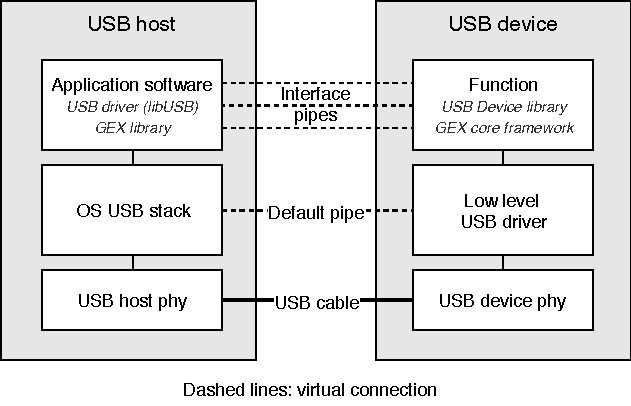
\includegraphics[scale=1] {img/usb-logical-redraw.pdf}
	\caption{\label{fig:usb-logical}The logical structure of USB}
\end{figure}

Endpoints can be either unidirectional or bidirectional; the direction from the host to a function is called OUT, the other direction (function the host) is called IN. A bidirectional endpoint is technically composed of a IN and OUT endpoint with the same number. All transactions (both IN and OUT) are initiated by the host; functions have to wait for their turn. Endpoint 0 is bidirectional, always enabled, and serves as a \textit{control endpoint}. The host uses the control endpoint to read information about the device and configure it as needed.

\subsection{Transfer Types}

There are four types of data transfers defined in \gls{USB}: control, bulk, isochronous, and interrupt. Each endpoint is configured for a fixed transfer type:

\begin{itemize}
	\item \textit{Control} - initial configuration after device plug-in; also used for other aplication-specific control messages that can affect other pipes.
	\item \textit{Bulk} - used for burst transfers of large messages, commonly e.g. for mass storage devices
	\item \textit{Isochronous} - streaming with guaranteed low latency; designed for audio or video streams where some data loss is preferred over stuttering
	\item \textit{Interrupt} - low latency short messages, used for human interface devices like mice and keyboards
\end{itemize}

\subsection{Interfaces and Classes}

The function's endpoints are grouped into \textit{interfaces}. An interface describes a logical connection of endpoints, such as the reception and transmission endpoints that belong together. An interface is assigned a \textit{class} defining how it should be used.

Standard classes are defined by the USB specification \cite{usb-class-list} to provide a uniform way of interfacing devices of the same type, such as human-interface devices (mice, keyboards, gamepads) or mass storage devices. The use of standard classes makes it possible to re-use the same driver software for devices from different manufacturers.

The class used for the GEX's ``virtual COM port'' function was originally meant for telephone modems, a common way of connecting to the Internet at the time the first versions of USB were developed. A device using this class will show as \verb|/dev/ttyACM0| on Linux and as a COM port on Windows, provided the system supports it natively or the right driver is installed.

\subsection{Descriptors}

USB devices are introspectable, that is, the host can learn about a newly connected device automatically by probing it, without any user interaction. This is accomplished using a \textit{descriptor table}, a binary structure stored in the function and read by the host through the control endpoint (default pipe) after the device is attached.

Each descriptor starts with a declaration of its length (in bytes), followed by its type,  allowing the host to skip unknown descriptors without having to discard the rest of the table. The descriptors are logically nested and form a tree-like structure, but they are stored sequentially in the descriptor table and the lengths do no include sub-descriptors.

The topmost descriptor holds information about the entire function, including the vendor and product IDs which uniquely identifies the device model. It is followed by a Configuration descriptor, grouping a set of interfaces. More than one configuration may be present and available for the host to choose from; however, this is rarely used or needed. Each configuration descriptor is followed by one or more interface descriptors, each with its class-specific sub-descriptors and/or endpoint descriptors.

The descriptor table used by GEX is captured in figure \ref{fig:gex-descriptors} for illustration. The vendor and product IDs were obtained from the pid.codes repository \cite{pidcodes} providing free product codes to open source projects. The official way of obtaining the unique code involves high recurring fees (\$4000 per annum) to the USB Implementers Forum, Inc. and is therefore not affordable for non-commercial use; alternatively, a product code may be obtained from some \gls{MCU} vendors if their product is used in the device.
\newpage

\hspace*{-1.5em}
\begin{minipage}[t]{0.5\textwidth}\scriptsize
\begin{verbatim}
Device Descriptor:
  bLength                18
  bDescriptorType         1
  bcdUSB               2.00
  bDeviceClass          239 Miscellaneous Device
  bDeviceSubClass         2 
  bDeviceProtocol         1 Interface Association
  bMaxPacketSize0        64
  idVendor           0x0483 STMicroelectronics
  idProduct          0x572a 
  bcdDevice            0.01
  iManufacturer           1 MightyPork
  iProduct                2 GEX
  iSerial                 3 0029002F-42365711-32353530
  bNumConfigurations      1
  Configuration Descriptor:
    bLength                 9
    bDescriptorType         2
    wTotalLength           98
    bNumInterfaces          3
    bConfigurationValue     1
    iConfiguration          0 
    bmAttributes         0x80
      (Bus Powered)
    MaxPower              500mA
    Interface Descriptor:
      bLength                 9
      bDescriptorType         4
      bInterfaceNumber        0
      bAlternateSetting       0
      bNumEndpoints           2
      bInterfaceClass         8 Mass Storage
      bInterfaceSubClass      6 SCSI
      bInterfaceProtocol     80 Bulk-Only
      iInterface              4 Settings VFS
      Endpoint Descriptor:
        bLength                 7
        bDescriptorType         5
        bEndpointAddress     0x81  EP 1 IN
        bmAttributes            2
          Transfer Type            Bulk
          Synch Type               None
          Usage Type               Data
        wMaxPacketSize     0x0040  1x 64 bytes
        bInterval               0
      Endpoint Descriptor:
        bLength                 7
        bDescriptorType         5
        bEndpointAddress     0x01  EP 1 OUT
        bmAttributes            2
          Transfer Type            Bulk
          Synch Type               None
          Usage Type               Data
        wMaxPacketSize     0x0040  1x 64 bytes
        bInterval               0
    Interface Association:
      bLength                 8
      bDescriptorType        11
      bFirstInterface         1
      bInterfaceCount         2
      bFunctionClass          2 Communications
      bFunctionSubClass       2 Abstract (modem)
      bFunctionProtocol       1 AT-commands (v.25ter)
      iFunction               5 Virtual Comport ACM
\end{verbatim}
\end{minipage}\hspace{1em}
\begin{minipage}[t]{0.5\textwidth}\scriptsize
\begin{verbatim}
    Interface Descriptor:
      bLength                 9
      bDescriptorType         4
      bInterfaceNumber        1
      bAlternateSetting       0
      bNumEndpoints           1
      bInterfaceClass         2 Communications
      bInterfaceSubClass      2 Abstract (modem)
      bInterfaceProtocol      1 AT-commands (v.25ter)
      iInterface              5 Virtual Comport ACM
      CDC Header:
        bcdCDC               1.10
      CDC Call Management:
        bmCapabilities       0x00
        bDataInterface          2
      CDC ACM:
        bmCapabilities       0x06
          sends break
          line coding and serial state
      CDC Union:
        bMasterInterface        1
        bSlaveInterface         2 
      Endpoint Descriptor:
        bLength                 7
        bDescriptorType         5
        bEndpointAddress     0x83  EP 3 IN
        bmAttributes            3
          Transfer Type            Interrupt
          Synch Type               None
          Usage Type               Data
        wMaxPacketSize     0x0008  1x 8 bytes
        bInterval             255
    Interface Descriptor:
      bLength                 9
      bDescriptorType         4
      bInterfaceNumber        2
      bAlternateSetting       0
      bNumEndpoints           2
      bInterfaceClass        10 CDC Data
      bInterfaceSubClass      0 
      bInterfaceProtocol      0 
      iInterface              6 Virtual Comport CDC
      Endpoint Descriptor:
        bLength                 7
        bDescriptorType         5
        bEndpointAddress     0x02  EP 2 OUT
        bmAttributes            2
          Transfer Type            Bulk
          Synch Type               None
          Usage Type               Data
        wMaxPacketSize     0x0040  1x 64 bytes
        bInterval               0
      Endpoint Descriptor:
        bLength                 7
        bDescriptorType         5
        bEndpointAddress     0x82  EP 2 IN
        bmAttributes            2
          Transfer Type            Bulk
          Synch Type               None
          Usage Type               Data
        wMaxPacketSize     0x0040  1x 64 bytes
        bInterval               0
\end{verbatim}
\end{minipage}\vspace{-1em}
\begin{figure}[H]
	\cprotect\caption{USB descriptors of a GEX prototype obtained using \verb|lsusb -vd vid:pid|}
\end{figure}


\section{USB Physical Layer}

\gls{USB} uses differential signaling with \gls{NRZI} encoding and bit stuffing (the insertion of dummy bits to prevent long intervals in the same \gls{DC} level). The encoding, together with frame formatting, checksum verification, retransmission, and other low-level aspects of the \gls{USB} connection are entirely handled by the \gls{USB} physical interface block in the microcontroller's silicon. Normally we do not need to worry about those details; nonetheless, a curious reader may find more information in chapters 7 and 8 of \cite{usbif-spec}. What needs our attention are the electrical characteristics of the physical connection, which need to be understood correctly for a successful schematic and \gls{PCB} design.

The \gls{USB} cable contains 4 conductors: V$_\mathrm{BUS}$ (+5\,V), D+, D--, and \gls{GND}. The data lines, D+ and D--, are also commonly labeled DP and DM. This differential pair should be routed in parallel on the \gls{PCB} and kept at the same length.

\gls{USB} versions that share the same connector are backwards compatible. The desired bus speed is requested by the device using a 1.5\,k$\Omega$ pull-up resistor to 3.3\,V on one of the data lines: D+ pulled high for Full Speed (shown in figure \ref{fig:usb-pullup-fs}), D-- pulled high for Low Speed. The polarity of the differential signals is also inverted depending on the used speed, as the idle level changes. Some microcontrollers integrate the correct pull-up resistor inside the \gls{USB} peripheral block (including out STM32F072), removing the need for an external resistor.

\begin{figure}[h]
	\centering
	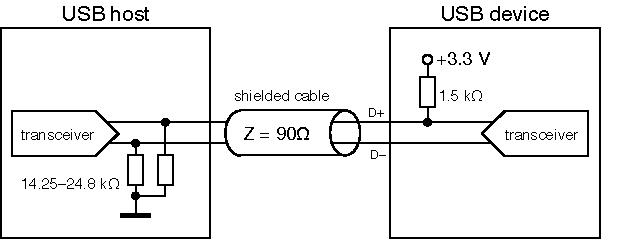
\includegraphics[scale=1]{img/usb-resistors.pdf}
	\caption[USB pull-ups]{\label{fig:usb-pullup-fs}Pull-up and pull-down resistors near the host and a Full Speed function, as prescribed by the USB specification rev. 2.0}
\end{figure}

When a function needs to be re-enumerated by the host, which causes a reload of the descriptor table and the re-attachment of software drivers, it can momentarily remove the pull-up resistor, which the host will interpret as if the device was disconnected. With an internal pull-up, this can be done by flipping a bit in a control register. An external resistor may be connected through a transistor controlled by a \gls{GPIO} pin. As discussed in \cite{eev-gpio-pu}, a GPIO pin might be used to drive the pull-up directly, though this has not been verified by the author.

The V$_\mathrm{BUS}$ line supplies power to \textit{bus-powered} devices. \textit{Self-powered} devices can leave this pin unconnected and instead use an external power supply. The maximal current drawn from the V$_\mathrm{BUS}$ line is configured using a descriptor and should not be exceeded, but experiments suggest this is often not enforced.

\noindent More details about the electrical and physical connection may be found in \cite{usb-nutshell}, sections \textit{Connectors} through \textit{Power}. 

\section{USB Classes}

This section explains the classes used in the GEX firmware. A list of all standard classes with a more detailed explanation can be found in \cite{usb-class-list}.

\subsection{Mass Storage Class} \label{sec:msc}

The \gls{MSC} is supported by all modern operating systems (MS Windows, MacOS, GNU/Linux, FreeBSD etc.) to support thumb drives, external disks, memory card readers and other storage devices.

%http://www.usb.org/developers/docs/devclass_docs/Mass_Storage_Specification_Overview_v1.4_2-19-2010.pdf
%http://www.usb.org/developers/docs/devclass_docs/usbmassbulk_10.pdf

The \gls{MSC} specification \cite{usbif-msco} defines multiple \textit{transport protocols} that can be selected using the descriptors. The \gls{BOT} \cite{usbif-bot} will be used for its simplicity. \gls{BOT} uses two bulk endpoints for reading and writing blocks of data and for the exchange of control commands and status messages. 

For the mass storage device to be recognized by the host operating system, it must also implement a \textit{command set}. Most mass storage devices use the \textit{\gls{SCSI} Transparent command set}
\footnote{To confirm this assertion, the descriptors of five thumb drives and an external hard disk were analyzed using \verb|lsusb|. All but one device used the SCSI command set, one (the oldest thumb drive) used \textit{SFF-8070i}. A list of possible command sets can be found in \cite{usbif-msco}}. 

Unfortunately, the \gls{SCSI} Transparent command set appears to have been deliberately left unspecified for license or copyright reasons (see discussion in \cite{usb-tscsi-wtf} and the surrounding thread) and the protocol now used under this name is an industry standard without a clear definition. Some pointers may be found in \cite{usb-tscsi} and by examining the source code of the USB Device driver library provided by ST Microelectronics.

This command set lets the host read information about the attached storage, such as its capacity, and check for media presence and readiness to write or detach. This is used e.g. for the ``Safely Remove'' function, which ensures that all internal buffers have been written to Flash.

In order to emulate a mass storage device without having a physical storage medium, we need to generate and parse the file system on-the-fly as the host \gls{OS} tries to access it. This will be discussed in chapter \ref{sec:fat16}.

\subsection{CDC/ACM Class} \label{sec:cdc-acm}

%https://www.keil.com/pack/doc/mw/USB/html/group__usbd__cdc_functions__acm.html

Historically meant for modem communication, \gls{CDCACM} is now the de facto standard way of making \gls{USB} devices appear as serial ports on the host \gls{OS}. Its specification can be found in \cite{usbif-cdc}. \gls{CDCACM} is a combination of two related classes, \gls{CDC} handling the data communication and \gls{ACM}, which defines control commands. Three endpoints are used: bulk IN, bulk OUT, and interrupt OUT.

The interrupt endpoint is used for control commands, such as toggling the auxiliary lines of RS-232 or setting the baud rate. Since GEX does not translate the data communication to any physical UART, those commands are not applicable and can be silently ignored.

An interesting property of the \gls{CDC} class is that the bulk endpoints transport raw data without any wrapping frames. By changing the interface's class in the descriptor table to 255 (\textit{Vendor Specific Class}), we can retain the messaging functionality of the designated endpoints, while accessing the endpoints device directly using e.g. libUSB, without any interference from the \gls{OS}. This approach is also used to hide the \gls{MSC} interface when its not needed.

\subsection{Interface Association: Composite Class}

The original \gls{USB} specification expected that each function will have only one interface enabled at a time. After it became apparent that there is a need to have multiple unrelated interfaces working in parallel, the \gls{IAD} \cite{usbif-iad} was introduced as a workaround.

The \gls{IAD} is an entry in the descriptor table that defines which interfaces belong together and should be handled by the same software driver. To use the \gls{IAD}, the function's class must be set to 239 (0xEF), subclass 2 and protocol 1 in the top level descriptor, so that the \gls{OS} knows to look for this descriptor before binding drivers to any interfaces.

In GEX, the \gls{IAD} is used to tie together the \gls{CDC} and \gls{ACM} interfaces while leaving out the \gls{MSC} interface which should be handled by a different driver. To make this work, a new \textit{composite class} had to be created as a wrapper for the library-provided \gls{MSC} and \gls{CDCACM} implementation.


\chapter{FreeRTOS}

FreeRTOS is a free, open-source real time operating system kernel that has been ported to over 30 microcontroller architectures. The kernel provides a scheduler and implements queues, semaphores and mutexes that are used for message passing between concurrent tasks and for synchronization. FreeRTOS is compact designed to be easy to understand; it's written in C with the exception of some architecture-specific routines that use assembly.

FreeRTOS is used in GEX for its synchronization objects and queues that make it easy to safely pass messages from USB interrupts to a working thread that processes them and sends back responses. Similar mechanism is used to handle external interrupts.

\section{Basic FreeRTOS Concepts and Functions}

\subsection{Tasks}

Threads in FreeRTOS are called \textit{tasks}. Each task is assigned a memory area to use as its stack space, and a structure with it's name, saved context and other metadata used by the kernel. A context includes the program counter, stack pointer and other register values. Task switching is done by saving and restoring this context by manipulating the values on stack before leaving and interrupt.

At start-up the firmware initializes the kernel, registers tasks to run and starts the scheduler. From this point onward the scheduler is in control and runs the tasks using a round robin scheme. Which task should run is primarily determined by their priority numbers, but there are other factors. FreeRTOS supports both static and dynamic object creation, including registering new tasks at run-time.

\subsubsection{Task Run States}

Tasks can be in one of four states: Suspended, Ready, Blocked, Running. The Suspended state does not normally occur in a task's life cycle, it's entered and left using API calls on demand. A task is in the Ready state when it can run, but is currently paused because a higher priority task is running. It enters the Running state when the scheduler switches to it. A Running task can wait for a synchronization object (e.g. a mutex) to be available. At this point it enters a Blocked state and the scheduler runs the next Ready task. When no tasks can run, the Idle Task takes control; it can either enter a sleep state to save power, or wait in an infinite loop until another task is available.

\subsubsection{Task Switching and Interrupts}

Task switching occurs periodically in a SysTick interrupt, usually every 1\,ms. After one tick of run time, the running task is paused (enters Ready state), or continues to run if no higher priority task is available. If a high priority task waits for an object and this is made available in an interrupt, the previously running task is paused and the waiting task is resumed immediately (enters the Running state). 

Only a subset of the FreeRTOS \gls{API} can be accessed from interrupt routines, for example it's not possible to use the delay function or wait for an object with a timeout, because the SysTick interrupt which increments the tick counter has the lowest priority and couldn't run. This is by design to prevent unexpected context switching in nested interrupts.

FreeRTOS uses a \textit{priority inheritance} mechanism to prevent situations where a high priority task waits for an object held by a lower priority task (called \textit{priority inversion}). The blocking task's priority is temporarily raised to the level of the blocked high priority task so it can finish faster and release the held object. Its priority is then degraded back to the original value. When the lower priority task itself is blocked, the same process can be repeated.

\subsection{Synchronization Objects}

FreeRTOS provides binary and counting semaphores, mutexes and queues. 

Binary semaphores can be used for task notifications, e.g. a task waits for a semaphore to be set by an interrupt when a byte is received on the serial port. This makes the task Ready and if it has a higher priority than the previously running task, it's immediately resumed to process the event.

Counting semaphores are used to represent available resources. A pool of resources (e.g. \gls{DMA} channels) is accompanied by a counting semaphore, so that tasks can wait for a resource to become available in the pool and then subtract the semaphore value. After finishing with a resource, the semaphore is incremented again and another task can use it.

Mutexes, unlike semaphores, must be taken and released in the same thread (task). They're used to guard exclusive access to a resource, such as transmitting on the serial port. When a mutex is taken, a task that wishes to use it enters Blocked state and is resumed once the mutex becomes available and it can take it.

Queues are used for passing messages between tasks, or from interrupts to tasks. Both sending and receiving queue messages can block until the operation becomes possible. 

In GEX, mutexes and semaphores are used for sending messages to the \gls{PC}, and a queue is used for processing received bytes and to send messages from interrupts, because it's not possible to block on a mutex or semaphore while inside an interrupt routine.

% TODO diagrams, figures


\chapter{The FAT16 File System and Its Emulation} \label{sec:fat16}

A \gls{FS} is used by GEX to provide a comfortable access to the configuration files. By emulating a Mass Storage \gls{USB} device, the module appears as a thumb drive on the host \gls{PC}, and the user can edit its configuration using their preferred text editor. The FAT16 file system was selected for its simplicity and a good cross-platform support \cite{os-support-table}.

Three variants of the \gls{FAT} file system exist: FAT12, FAT16, and FAT32. FAT12 was used on floppy disks and it is similar to FAT16, except for additional size constraints and a \gls{FAT} entry packing scheme. FAT16 and FAT32 are FAT12's later developments from the time when hard disks became more common and the old addressing scheme could not support their larger capacity.

This chapter will explain the structure of FAT16 and the challenges faced when trying to emulate it without a physical data storage.

\section{The General Structure of the FAT File System}

An overview will be presented here without going into too many details that would overwhelm the reader and can be looked up elsewhere. Several resources \cite{ms-fat,fat16-brainy,fat16-maverick,fat16-phobos,fat-whitepaper} were consulted during the development of the GEX firmware which provide a more complete description of the FAT16 file system, with \cite{fat-whitepaper}, the Microsoft white paper, giving the most detailed overview.

The storage medium is organized into \textit{sectors} (or \textit{blocks}), usually 512 bytes long. Those are the smallest addressing unit in the disk structure. The disk starts with a \textit{boot sector}, also called a \gls{MBR}). That is followed by optional reserved sectors, one or two copies of the file allocation table, and the root directory. All disk areas are aligned to a sector boundary:

\begin{table}[h]
	\centering
	\begin{tabular}{ll}
		\toprule
		\textbf{Disk area} & \textbf{Size / Notes} \\
		\midrule
		Boot sector & 1 sector \\
		Reserved sectors & optional \\
		FAT 1 & 1 or more sectors, depends on disk size \\
		FAT 2 & optional, a back-up copy of FAT 1 \\
		Root directory & 1 or more sectors \\
		Data area & Organized in \textit{clusters} \\
		\bottomrule
	\end{tabular}
	\caption{\label{tab:fat16-disk-areas}Areas of a FAT-formatted disk}
\end{table}

\subsection{Boot Sector}

This is a 1-sector structure which holds the \gls{OS} bootstrap code for bootable disks. The first 3 bytes are a jump instruction to the actual bootstrap code located later in the sector. What matters to us when implementing the file system is that the boot sector also contains data fields describing how the disk is organized, what file system is used, who formatted it, etc. The size of the \gls{FAT} and the root directory is defined here. The exact structure of the boot sector can be found in either of \cite{ms-fat,fat16-brainy,fat16-maverick,fat16-phobos,fat-whitepaper} or in the attached GEX source code.

\subsection{File Allocation Table}

The data area of the disk is organized in clusters, logical allocation units composed of groups of sectors. The use of a larger allocation unit allows the system to use shorter addresses and thus support a larger disk capacity.

The \gls{FAT} acts as a look-up table combined with linked lists. In FAT16, it is organized in 16-bit fields, each corresponding to one cluster. The first two entries in the allocation table are reserved and hold special values set by the disk formatter and the host \gls{OS}: a ``media descriptor'' 0xFFF8 and a ``clean/dirty flag'' 0xFFFF/0x3FFF.

Files can span multiple clusters; each \gls{FAT} entry either holds the address of the following file cluster, or a special value:

\begin{itemize}[nosep]
	\item 0x0000 - free cluster
	\item 0xFFFF - last cluster of the file (still including file data)
	\item 0xFFF7 - bad cluster
\end{itemize}

The bad cluster mark, 0xFFF7, is used for clusters which are known to corrupt data due to a flaw in the storage medium, such us a bad memory cell.

\subsection{Root Directory}

The root directory has the same structure as any other directories, which reside in clusters the same way like ordinary files. The difference is that the root directory is allocated when the disk is formatted and it has a fixed and known position and size. Sub-directories are stored on the disk in a way similar to regular files, therefore they can span multiple sectors and their file count can be much larger than that of the root directory.

\begin{table}
	\centering
	\begin{tabular}{lll}
		\toprule
		\textbf{Offset} & \textbf{Size (bytes)}  & \textbf{Description}\\
		\midrule
		0 & 8 & File name (padded with spaces) \\
		8 & 3 & File extension \\
		11 & 1 & File attributes \\
		12 & 10 & Reserved \\
		22 & 2 & Creation time \\
		24 & 2 & Creation date \\
		26 & 2 & Address of the first cluster \\
		28 & 4 & File size (bytes) \\
		\bottomrule
	\end{tabular}
	\caption{\label{tab:fat16-dir-entry}Structure of a FAT16 directory entry}
\end{table}

A directory is organized in 32-byte entries representing individual files. Table \ref{tab:fat16-dir-entry} shows the structure of one such entry. The name and extension fields form together the well-known 8.3 filename format (referring to the byte size of the first two entries). Longer file names are encoded using a \gls{LFN} scheme \cite{fat-lfn} as special hidden entries stored in the directory table alongside the regular 8.3 entries, ensuring backward compatibility.

\noindent
The first byte of the file name has a special meaning:

\begin{itemize}
	\item 0x00 - indicates that there are no more files when searching the directory
	\item 0xE5 - marks a free slot; this is used when a file is deleted
	\item 0x05 - indicates that the first byte should actually be 0xE5, a code used in some character sets at the time, and the slot is \textit{not} free\footnote{The special meaning of 0xE5 appears to be a correction of a less than ideal design choice earlier in the development of the file system}.
	\item Any other value, except 0x20 (space) and characters forbidden in a DOS file name, starts a valid file entry. Generally, only space, A-Z, 0-9, \verb|-| and \verb|_| should be used in file names for maximum compatibility.
\end{itemize}

The attributes field contains flags such as \textit{directory}, \textit{volume label}, \textit{read-only} and \textit{hidden}. Volume label is a special entry in the root directory, which defines the disk's label shown on the host \gls{PC}. A file with the directory bit set is actually a pointer to a subdirectory, meaning that when we open the linked cluster, we'll find a new directory table.

Figure \ref{fig:fat-example} shows a possible organization of the GEX file system with two INI files, one spanning two clusters, the other being entirely inside one. The clusters need not be used completely; an exact file size is stored in the directory entries.

\begin{figure}[h]
	\centering
	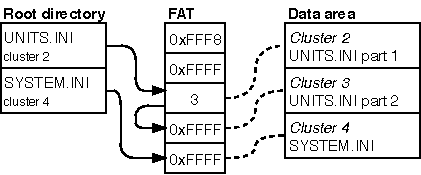
\includegraphics[scale=1.3] {img/fat-links.pdf}
	\caption{\label{fig:fat-example}An example of the GEX virtual file system}
\end{figure}


\section{FAT16 Emulation}

The FAT16 file system is relatively straightforward to implement. However, it is not practical or even possible to keep the entire file system in memory on a small microcontroller like our STM32F072. This means that we have to generate and parse disk sectors and clusters on-demand, when the host reads or writes them. The STM32 \gls{USB} Device library helpfully implements the \gls{MSC} and provides \gls{API} endpoints to which we connect our file system emulator. Specifically, those are requests to read and write a sector, and to read disk status and parameters, such as its size.

\subsection{DAPLink Emulator}

A FAT16 emulator was developed as part of the open-source Arm Mbed DAPLink project \cite{daplink}. It is used there for a drag-and-drop flashing of firmware images to the target microcontroller, taking advantage of the inherent cross-platform support (it uses the same software driver as any thumb drive, as discussed in \ref{sec:msc}). Arm Mbed also uses a browser-based \gls{IDE} and cloud build servers, thus the end user does not need to install or set up any software to program a compatible development kit.

The GEX firmware adapts several parts of the DAPLink code, optimizing its \gls{RAM} usage and porting it to work with FreeRTOS. Those modified files are located in the folder \mono{User/vfs} of the GEX source code repository; the original Apache 2.0 open source software license headers, as well as file names, have been retained.

\subsection{Handling a Read Access}

As shown in table \ref{tab:fat16-disk-areas}, the disk consists of several areas. The boot sector is immutable and can be stored in and read from the Flash memory. The handling of the other disk areas (\gls{FAT}, data area) depends on the type of access: read or write.

The user can only read files that already exist on the disk, in our case, \verb|UNITS.INI| and \verb|SYSTEM.INI|. Those files are generated from the binary settings storage, and conversely, parsed, line-by-line, without ever existing in their full form. This fact makes our task more challenging, as the files cannot be easily measured and there's no obvious way to read a sector from the middle of a longer file. We solve this by implementing two additional functions in the INI file writer: a \textit{read window} and a \textit{dummy read mode}.

A read window is a byte range which we wish to generate. The INI writer discards bytes before the start of the read window, writes those inside the window to our data buffer, and stops when its end is reached. This lets us extract a sector from anywhere in a file. The second function, dummy read, is tied to the window function: we set the start index so high that it is never reached (e.g. 0xFFFFFFFF), and have the writer count discarded characters. When the dummy file generation ends, this character counter holds its size.

Now, just one problem remains: how to tell which sectors contain which part of our files? This is straightforward when we realize that the files change only when the user modifies the settings. After each such change, an algorithm is run which allocates clusters to the files and preserves this information in a holding structure. A subsequent read access simply requires a look into this structure and the corresponding chunk of a file may be served using the read window function. The \gls{FAT} can be dynamically generated from this information as well.

\subsection{Handling a Write Access}

A write access to the disk is more challenging to emulate than a read access, as the host OS tends to be somewhat unpredictable. In GEX's case we are interested only in the action of overwriting an already existing file, but it is interesting to also analyze other actions the host may perform.

It must be noted that due to the nonexistence of a physical storage medium, it is not possible to read back a file the host has previously written, unless we store or re-generate its content when such a read access occurs. The \gls{OS} may show the written file on the disk, but when the user tried to read it, the action either fails, or shows a cached copy. The emulator woulds around this problem by temporarily reporting that the storage medium has been removed, forcing the host to re-load its contents.

\subsubsection{File Deletion}

A file is deleted by:

\begin{enumerate}
	\item Marking all sectors used by it as free in the \gls{FAT}
	\item Replacing the first character of its name in the directory table by 0xE5 to indicate the slot is free
\end{enumerate}

From the perspective of emulation, we can ignore the \gls{FAT} access and only detect writes to the directory sectors. This is slightly more complicated when one considers that all disk access is performed in sectors: the emulator must compare the written data with the original bytes to detect what change has been performed. Alternatively, we could parse the entire written sector as a directory table and compare it with our knowledge of its original contents.

\subsection{File Name Change}

A file is renamed by modifying its directory entry. In the simple case of a short, 8.3 file name, this is an in-place modification of the file entry. Long file names, using the \gls{LFN} extension, are a complication, as the number of non-file entries holding the long file name might change, and subsequently the following entries in the table may shift or be re-arranged.

\subsection{File Creation}

A new file is created in three steps:

\begin{enumerate}
	\item Finding free clusters and chaining them by writing the following cluster addresses (or 0xFFFF for the last cluster) into the \gls{FAT}
	\item Finding and overwriting a free entry in the directory table
	\item Writing the file content
\end{enumerate}

It can be expected the host \gls{OS} first finds the free sectors and a free file entry before performing any write operations, to prevent a potential disk corruption.

To properly handle such a file by the emulator, we could, in theory, find its name from the directory table, which has been updated, and then collect the data written to the corresponding clusters. In practice, confirmed by experiments with a real Linux host, those three steps may happen in any order, and often the content is written before the directory table is updated.

The uncertain order of the written disk areas poses a problem when the file name has any significance, as we cannot store the received file data while waiting for the name to be written. The DAPLink mbed flashing firmware solves this by analyzing the content of the first written sector of the file, which may contain the binary \gls{NVIC} table, or a character pattern typical for Intel hex files.

\subsection{File Content Change}

A change to a file's content is performed in a similar way to the creation of a new file, except instead of creating a new entry in the directory table, an existing one is updated with the new file size. The name of the file may be unknown until the content is written, but we could detect the file name by comparing the start sector with those of all files known to the virtual file system.

In the case of GEX, the detection of a file name is not important; we expect only INI files to be written, and the particular file may be detected by its first section marker, such as \verb|[UNITS]| or \verb|[SYSTEM]|. Should a non-INI file be written by accident, the INI parser will likely detect a syntax error and discard it.

It should be noted that a file could be updated only partially, skipping the clusters which remain unchanged, and there is also no guarantee regarding the order in which the file's sectors are written. This is hard to detect and handle correctly, but it can be detected by the emulator and such a write operation will be discarded. Fortunately, this host behavior has not been conclusively observed in practice, but the writing of a file rarely fails for unknown reasons; this could be a possible cause.













\chapter{Supported Hardware Buses}

\section{UART and USART}

The \textit{Universal Synchronous / Asynchronous Receiver Transmitter} has a long history and is still in widespread use today. It is the protocol used in RS-232, which was once a common way of connecting modems, printers, mice and other devices to personal computers. UART framing is also used in the industrial bus RS-485.

UART and USART are two variants of the same interface. USART includes a separate clock signal, while the UART timing relies on a well-known clock speed and the bit clock is synchronized by start bits. USART was historically used in modems to achieve higher bandwidth, but is now mostly obsolete.

USART, as implemented by microcontrollers such as the STM32 family, is a two-wire full duplex interface that uses 3.3\,V or 5\,V logic levels. The data lines are in the high logical level when idle. A frame, pictured in figure \ref{fig:uart-frame} starts by a start-bit (low level for the period of one bit) followed by \textit{n} data bits (typically eight), an optional parity bit and a period of high level called a stop bit or stop bits, usually between one and two bits long.

\begin{figure}
	\centering
	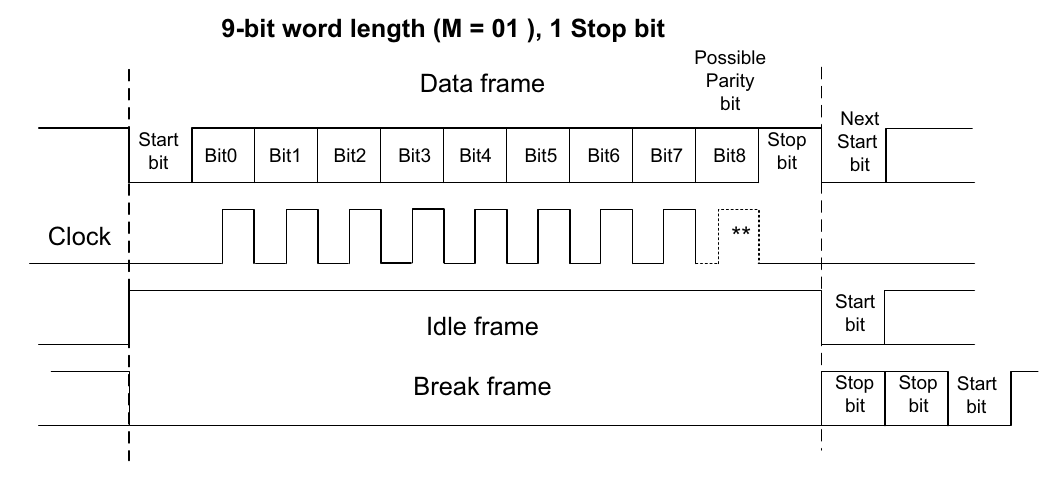
\includegraphics[width=.8\textwidth] {img/usart.png}
	\caption{\label{fig:uart-frame}UART frame, as shown by the STM32F072 Reference Manual. Break frames are used by some UART based protocols, like LIN (Local Interconnect Network).}
\end{figure}
 
RS-232 uses the UART framing, but its logic levels are different: logical 1 is represented by negative voltages $-3$ to $-25$\,V and logical 0 uses the same range, but positive. To convert between RS232 levels and TTL (5\,V) levels, a level-shifting circuit such as the MAX232 can be used. In RS232, the two data lines (Rx and Tx) are accompanied by RTS (Ready To Send), CTS (Clear To Send) and DTR (Data Terminal Ready) which facilitate handshaking and hardware flow control. In practice, those additional signals are often unused or their function differs; for instance, Arduino boards (using a USB-serial converter) use the DTR line as a reset signal to automatically enter their bootloader for firmware flashing.

\todo[inline]{examples}

\section{SPI}

SPI (Serial Peripheral Interface) is a point-to-point or multi-drop master-slave interface based on shift registers. The SPI connection with multiple slave devices is depicted in figure \ref{fig:spi-multislave}. It uses at least 4 wires: SCK (Serial Clock), MOSI (Master Out Slave In), MISO (Master In Slave Out) and SS (Slave Select). SS is often marked CSB (Chip Select Bar) or NSS (Negated Slave Select) to indicate it's active low. Slave devices are addressed using their Slave Select input while the data connections are shared. A slave that's not addressed releases the MISO line to a high impedance state so it doesn't interfere in ongoing communication.

Transmission and reception on the SPI bus happen simultaneously. A bus master asserts the SS pin of a slave it wishes to address and then sends data on the MOSI line while receiving a response on MISO. It's customary that the slave responds with zeros or a status byte as the first byte of the response.

SPI devices often provide a number of control, configuration and status registers that can be read and written by the bus master. The first byte of a command usually contains one bit that determines if it's a read or write access, and an address field selecting the target register.

\begin{figure}
	\centering
	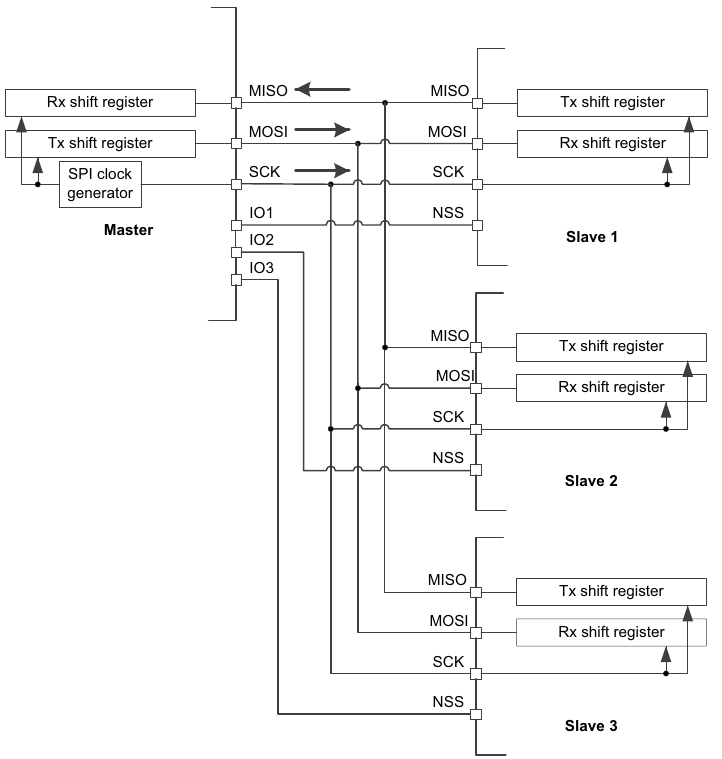
\includegraphics[width=.9\textwidth] {img/spi-multislave.png}
	\caption{\label{fig:spi-multislave}A SPI bus with 1 master and 3 slaves, each enabled by its own Slave Select signal (\textit{STM32F072 Reference Manual})}
\end{figure}

\todo[inline]{examples}

\section{I2C}

I2C is a two-wire (SDA--\textit{Serial Data}, SCL--\textit{Serial Clock}), open-drain bus that supports multi-master operation. The protocol was developed by Philips Semiconductor (now NXP Semiconductors) and until 2006 implementors were required to pay licensing fees, leading to the development of compatible implementations with different names, such as Atmel's Two Wire Interface (TWI). I2C is the basis of the SMBus and PMBus protocols which add additional constraints and rules for a more robust operation.

I2C uses two addressing modes: 7-bit and 10-bit. Due to the small address space, exacerbated by many devices implementing only the 7-bit addressing, collisions between chips from different manufacturers are common; many devices thus offer several pins to let the board designer choose a few bits of the address by connecting them to different logic levels. I2C allows slow slave devices to stop the master from sending more data by holding the SCL line low at the end of a byte. As the bus is open-drain, the line can't go high until all participants release it. This function is called \textit{Clock Stretching}.

\begin{figure}
	\centering
	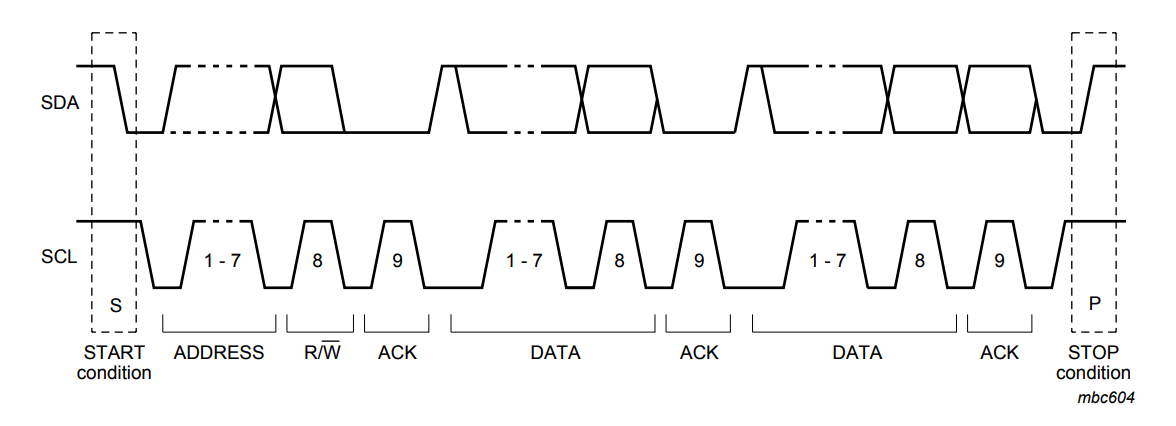
\includegraphics[width=.9\textwidth] {img/i2c-frame.png}
	\caption{\label{fig:i2c-frame}An I2C message. The frame starts with a start condition and stops with a stop condition, defined by an SDA edge while SCL is high. The address and data bytes are acknowledged by the slave by sending a 0 on the open-drain SDA line in the following clock cycle. A slave can terminate the transaction by sending 1 in place of the acknowledge bit. (\textit{Diagram taken from the I2C specification UM10204 by NXP Semiconductors})}
\end{figure}

The bus supports multi-master operation, which leads to the problem of collisions. Multi-master capable devices must implement a bus arbitration scheme as specified by the I2C standard. This feature is not often used in intelligent sensors and modules; the most common topology is multi-drop single-master, similar to SPI, with the advantage of using only two pins on the microcontroller.

\section{1-Wire}

The 1-Wire bus, developed by Dallas Semiconductor, uses a single bi-directional data line which can also power the slave devices, reducing the number of required wires to just two (compare with 3 in I2C and 5 in SPI, all including GND). 

1-Wire is open-drain and the communication consists of short pulses sent by the master and (for bit reading) the line continuing to be held low by the slave. The pulse timing (fig. \ref{fig:1w-pulses}) defines if it's a read or write operation and what bit value it carries. A transaction is started by a 480us long "reset" pulse send by master and ended by a 1-byte CRC checksum.

\begin{figure}
	\centering
	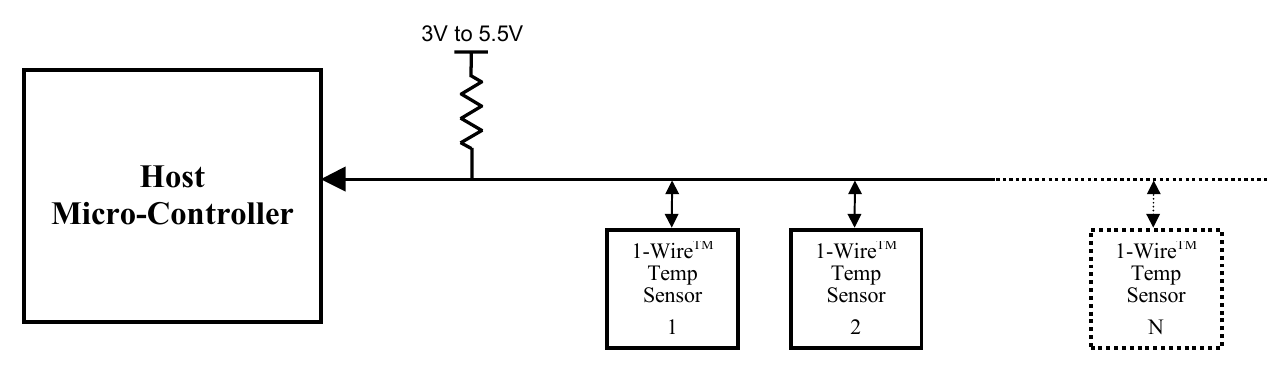
\includegraphics[width=.9\textwidth] {img/1w-topology.png}
	\caption{\label{fig:1w-topology}1-Wire topology (by \textit{Dallas Semiconductor})}
\end{figure}

\begin{figure}
\centering
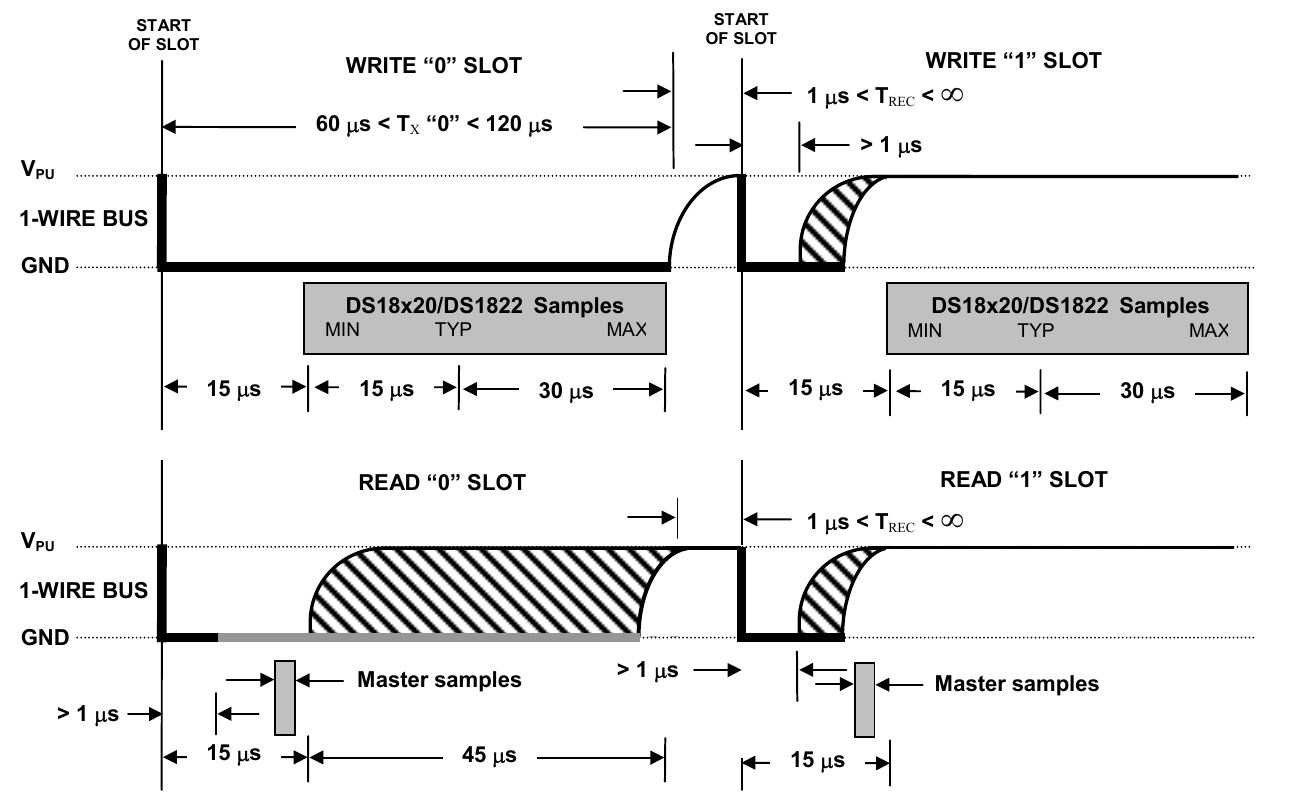
\includegraphics[width=\textwidth] {img/1w-rw.png}
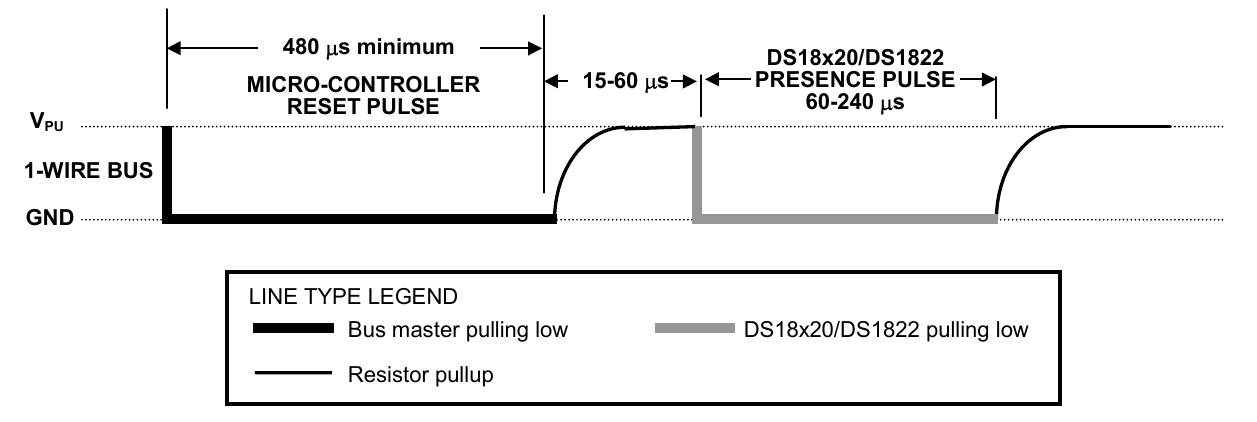
\includegraphics[width=\textwidth] {img/1w-reset.png}
\caption{\label{fig:1w-pulses}1-Wire DIO pulse timing (by \textit{Dallas Semiconductor})}
\end{figure}

1-Wire is a master-slave multi-drop bus. Devices are addressed by their unique 64-bit ID numbers (called ROMs); those IDs are found by the bus master with the cooperation from slaves using a ROM search protocol. If only one device is connected, a special command set can be used to skip addressing.

\section{NeoPixel}

NeoPixel is a marketing name of the WS2811, WS2812 and compatible intelligent LED drivers that is commonly used in "addressable LED strips". Those chips include the control logic, PWM drivers and usually the LED diodes all in one miniature package.

The NeoPixel protocol is unidirectional, using only one data pin. The LED drivers are chained together. Ones and zeros are encoded by a pulse length on the data pin; after loading the color data to the LED string, a longer "reset" pulse is issued by the bus master and the set colors are displayed.

The NeoPixel timing is very sensitive to pulse length accuracy. Reliable ways to implement it use DMA with a hardware timer, or a I2S peripheral. An easier method that does not use any additional hardware resources is implementing the protocol as delay loops in the firmware; care must be taken to disable interrupts in the sensitive parts of the timing.













\chapter{Non-communication Hardware Functions}

In addition to communication buses, described in \cref{ch:hw_buses}, GEX implements several measurement and output functions that take advantage of the microcontroller's peripheral blocks, such as timers/counters and \gls{DAC}. The more complicated ones are described here; simpler functions, such as the raw \gls{GPIO} access, will be described later together with their control \gls{API}.

\section{Frequency Measurement} \label{sec:theory-fcap}

Applications like motor speed measurement and the reading of a \gls{VCO} or \gls{VCO}-based sensor's output demand a tool capable of measuring frequency. This can be done using a laboratory instrument such as the Agilent 53131A. A low-cost solution can be realized using a timer/counter peripheral of a microcontroller.

\noindent
Two basic methods to measure frequency exist~\cite{fcap-twotypes}, each with its advantages and drawbacks:

\begin{itemize}
	\item The \textit{direct method} (\cref{fig:fcap-direct-dia}) is based on the definition of frequency as a number of cycles $n$ in a fixed-length time window $\tau$ (usually 1\,s); the frequency is then calculated as $f=n/\tau$.

	One timer generates the time window and its output gates the input of another, configured as a pulse counter. At the end of the measurement window an interrupt is generated and we can read the pulse count from the counter's register.

	The direct method has a resolution of 1\,Hz with a sampling window of 1\,s (only a whole number of pulses can me counted). The resolution can be increased by using a longer time window, provided the measured signal is stable enough to make averaging possible without distorting the result. Further increase of precision is possible through analog or digital interpolation~\cite{fcap-increasing}, a method used in some professional equipment.

	\item The \textit{indirect} or \textit{reciprocal method} (\cref{fig:fcap-reci-dia}) measures one period $T$ as the time interval between two pulses and this is then converted to frequency as $f=1/T$.

	This method needs only one timer/counter. Cycles of the system clock are counted for the duration of one period on the input pin (between two rising edges). If we additionally detect the falling edge in between, the counter's value gives us the duty cycle when related to the overall period length.

	Te reciprocal method's resolution depends on the counter's clock speed; if driven at 48\,MHz, the tick period is 20.83\,ns, which defines the granularity of our time measurement. It is common to measure several pulses and average the obtained values to further increase the precision.

	We can easily achieve a sub-hertz resolution with this method, but its performance degrades at high frequencies where the time measurement precision becomes insufficient. The input frequency range can be extended using a hardware prescaller\footnote{\textit{Prescaller} is a divider implemented as part of the timer/counter peripheral block that can be optionally enabled and configured to a desired division factor.}, which is also applicable to the direct method, should the measurement of frequencies outside the counter's supported range be required. A duty cycle measurement available in this method can be used to read the output of sensors that use a pulse-width modulation.

\end{itemize}

\begin{figure}[h]
	\centering
	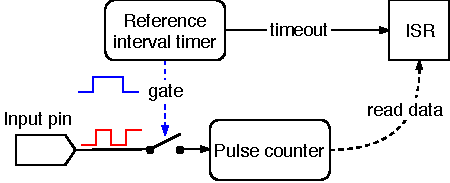
\includegraphics[scale=1] {img/fcap-direct.pdf}
	\caption{\label{fig:fcap-direct-dia}Direct frequency measurement method}
\end{figure}

\begin{figure}[h]
\centering
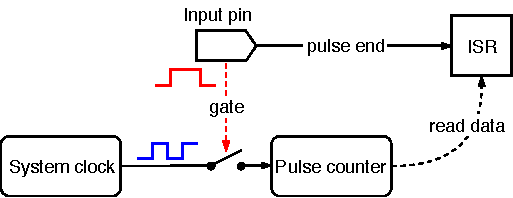
\includegraphics[scale=1] {img/fcap-reciprocal.pdf}
\caption{\label{fig:fcap-reci-dia}Reciprocal frequency measurement method}
\end{figure}

Which method to use depends on the frequency we want to measure; the worst-case measurement errors of both methods, assuming an ideal 48\,MHz system clock, are plotted in \cref{fig:freqmethods-graph}. It can be seen that the reciprocal method leads in performance up to 7\,kHz where the direct method overtakes it. If a higher error is acceptable, the reciprocal method could be used also for higher frequencies to avoid a reconfiguration and to take advantage of its higher speed.

\begin{figure}[h]
	\centering
	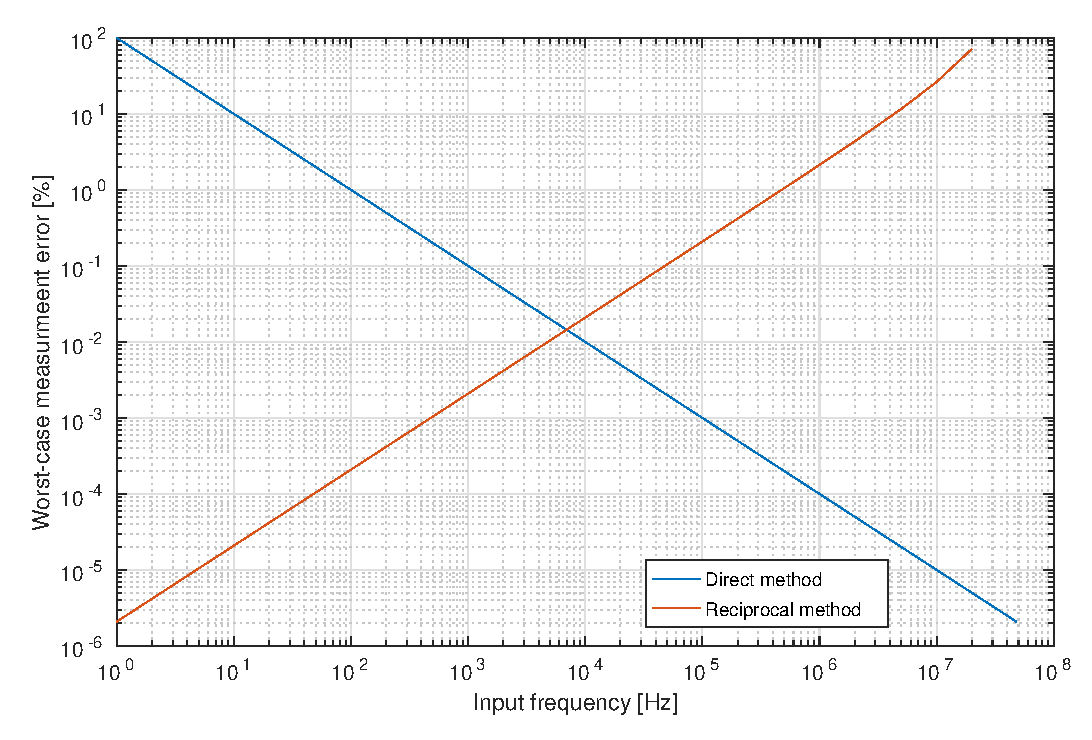
\includegraphics[width=\textwidth] {img/freqmethods.eps}
	\caption[Frequency measurement methods comparison]{\label{fig:freqmethods-graph}Worst-case error using the two frequency measurement methods with an ideal 48\,MHz timer clock. The crossing lies at 7\,kHz with an error of 0.015\,\%, or 1.05\,Hz.}
\end{figure}

A good approach to a universal measurement, for cases where we do not know the expected frequency beforehand, could be to obtain an estimate using the direct method first, and if the frequency is below the worst-case error crossing point (here 7\,kHz, according to \cref{fig:freqmethods-graph}), to take a more precise measurement using the reciprocal method.

The system clock's frequency, which we use to measure pulse lengths and to gate the pulse counter, will be affected by tolerances of the used components, the layout of the \gls{PCB}, temperature effects etc., causing measurement errors. A higher accuracy could be achieved using a \gls{TCO}, or, in the direct method, with the synchronization pulse provided by a \gls{GPS} receiver to time the measurement interval.

\section{Analog Signal Acquisition} \label{sec:theory-adc}

A very common need in experiments involving the measurement of physical properties is the acquisition of analog signals, respective voltages. Those can be roughly divided into \gls{DC} and \gls{AC} or time-changing signals. Analog signals are converted to digital values using \glspl{ADC}. Several principles of analog signal measurement exist with different cost, speed, resolution, and many other factors which determine their suitability for a particular application.

\gls{DC} signals can be measured by taking several samples and calculating their average value; in the presence of a 50\,Hz or 60\,Hz mains interference, its advisable to spread those samples over the 20\,ms (resp. 16.7\,ms) time of one period so that the interfering waveform cancels out. Time-changing signals can be captured by taking isochronous samples at a frequency conforming to the Nyquist theorem, that is, at least twice that of the measured signal. In practice, a frequency several times higher is preferred for a more accurate capture.

\begin{figure}
	\centering
	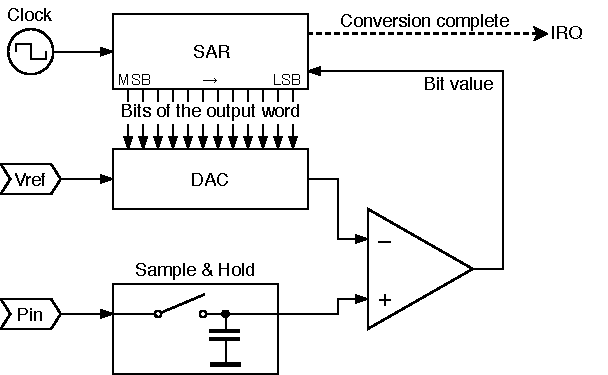
\includegraphics[scale=1] {img/sar-adc.pdf}
	\caption{\label{fig:adc-sar}A diagram of the SAR type ADC}
\end{figure}

The \gls{ADC} type commonly available in microcontrollers, including our STM32F072, uses a \textit{successive approximation} method. It is called the \textit{SAR type \gls{ADC}}, after its main component, the \gls{SAR}. A diagram of this \gls{ADC} is shown in \cref{fig:adc-sar}.

The \gls{SAR} type converter uses a \gls{DAC}, controlled by the value in the \gls{SAR}, which approximates the input voltage, bit by bit, following the algorithm described in~\cite{adc-sar} and outlined below:

\begin{enumerate}
	\item The \gls{SAR} is cleared to all zeros.
	\item The \gls{DAC} generates an approximation voltage.
	\item Its output is compared with the sampled input, and the comparator's output is stored as the active bit in the approximation register.
	\item The approximation continues with step 2 and the following (less significant) bit.
	\item When all bits of the data word were found, an interrupt request is generated and the application program can read it from the \gls{SAR}.
\end{enumerate}

A change of the input value would make this principle unreliable, which is why the input is buffered by a sample \& hold circuit. The holding capacitor is charged to the input voltage and maintains this level during the conversion. The duration for which the capacitor is connected to the input is called a \textit{sampling time}.

\section{Waveform Generation} \label{sec:theory-dac}

A waveform generator is a useful tool in many experiments and measurements. A sine stimulus is the basis of a lock-in amplifier; it can be used to measure impedance; with a frequency sweep, we can obtain the frequency response of an analog filter, etc. We can, of course, generate other waveforms, such as a triangle, ramp, or rectangle wave.

The \gls{DAC} peripheral can produce a \gls{DC} level on the output pin based on a control word. When we periodically change its digital input, it produces an analog waveform.

\subsection{Waveform Generation with DMA and a Timer} \label{sec:theory-dac-simple}

A straightforward, intuitive implementation of the waveform generator is illustrated in \cref{fig:wavegen-naive}. This approach has its advantages: it is simple and works autonomously, with no interrupt handling or interventions from the program. It could be implemented without the use of \gls{DMA} as well, using a loop periodically updating the \gls{DAC} values; of course, such approach is less flexible and we would run into problems with interrupt handling affecting the timing accuracy.

\begin{figure}[h]
	\centering
	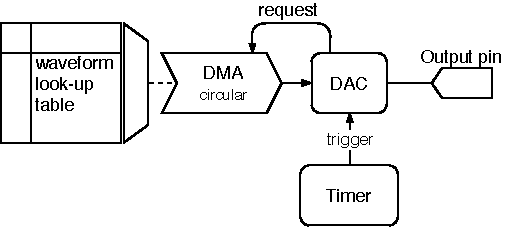
\includegraphics[scale=1.1] {img/wavegen-naive.pdf}
	\caption[A simple implementation of the waveform generator]{\label{fig:wavegen-naive}A simple implementation of the waveform generator, using DMA and a look-up table}
\end{figure}

The highest achievable output frequency largely depends on the size of our look-up table. For instance, assuming a timer frequency of 48\,MHz and a 8192-word table, holding one period of the waveform, the maximum frequency would be short of 6\,kHz, whereas if we shorten the table to just 1024 words, we can get almost 47\,kHz on the analog output. The downside of a shorter table is a lower resolution, which will appear as \gls{DC} plateaus or steps when observed with an oscilloscope, producing harmonic components similar to those of a square wave.

A major disadvantage of this simple generation method is given by the limitations of the used timer, which defines the output frequency. Its output trigger fires when the internal counter reaches a pre-defined value, after which the counting register is reset. The counting speed is derived from the system clock frequency $f_\mathrm{c}$ using a prescaller $P$ and the set maximum value $N$. Only output frequencies that can be exactly expressed as $f=f_\mathrm{c}/(P\cdot N \cdot \mathrm{TableSize})$ can be accurately produced. Still, this simple and efficient method may be used where fine tuning is not required to take advantage of its fully asynchronous operation.

\subsection{Direct Digital Synthesis} \label{sec:theory-dac-dds}

There are situations where the simple waveform generation method is not sufficient, particularly when a fine tuning or on-line frequency and phase changes are required. Those are the strengths of \gls{DDS}, an advanced digital waveform generation method well explained in~\cite{all-about-dds}.

\begin{figure}[h]
	\centering
	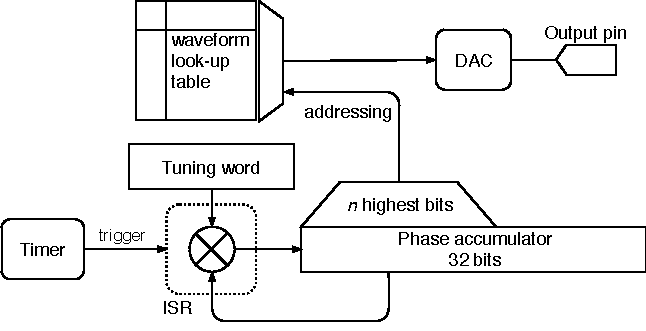
\includegraphics[scale=1] {img/wavegen-dds.pdf}
	\caption{\label{fig:wavegen-dds}A block diagram of a DDS-based waveform generator}
\end{figure}

A diagram of a possible \gls{DDS} implementation in the STM32 firmware is shown in \cref{fig:wavegen-dds}. It is based on a \gls{NCO}. The \gls{NCO} consists of a \textit{phase accumulator} register and a \textit{tuning word} which is periodically added to it at a constant rate in a timer interrupt handler. The value of the tuning word determines the output waveform frequency. The look-up table must have a power-of-two length so that it can be addressed by the \textit{n} most significant bits of the phase accumulator. An additional control word could be added to this address to implement a phase offset for applications like a phase-shift modulation.

The output frequency is calculated as \(f_\mathrm{out} = \dfrac{M\cdot f_\mathrm{c}}{2^n}\), where $M$ is the tuning word, $n$ is the bit length of the phase accumulator, and $f_c$ is the frequency of the phase-updating interrupt. The number of bits used to address the look-up table does not affect the output frequency; the table can be as large as the storage space allows. A tuning word value exceeding the lower part of the phase accumulator (including bits which directly enter the look-up address) will cause some values from the table to be skipped. A smaller tuning word, conversely, makes some values appear on the output more than once. This can be observed as steps or flat areas on the output. When the tuning word does not evenly divide $2^n$, that is, the modulo is non-zero, we can also observe jitter.

\subsubsection{DDS Implemented in Hardware}

DDS may be implemented in hardware, including the look-up table, often together with the \gls{DAC} itself, which is then called a \textit{Complete \gls{DDS}}. That is the case of e.g. AD9833 from Analog Devices. As the software implementation depends on a periodic interrupt, it is often advantageous to use a component like this when we need higher output frequencies where the use of an interrupt is not possible. GEX can control an external waveform generator like the AD9833 using an \gls{SPI} port.

\section{Touch Sensing} \label{sec:theory-touch}

The used microcontroller, STM32F072, includes a \gls{TSC} peripheral block. It can be accessed from GEX as a demonstration of capacitive touch sensing, and could possibly be used for simple touch sensors as well, such as measuring the level of water in a tank.

The TSC requires a specific topology with a sampling capacitor connected close to the microcontroller pin, which may not be possible on a universal GEX module; for this reason, the touch sensing feature is best demonstrated on the STM32F072 Discovery development kit, which includes a 4-segment touch slider shown in \cref{fig:disco-touch}.

\begin{figure}[h]
	\centering
	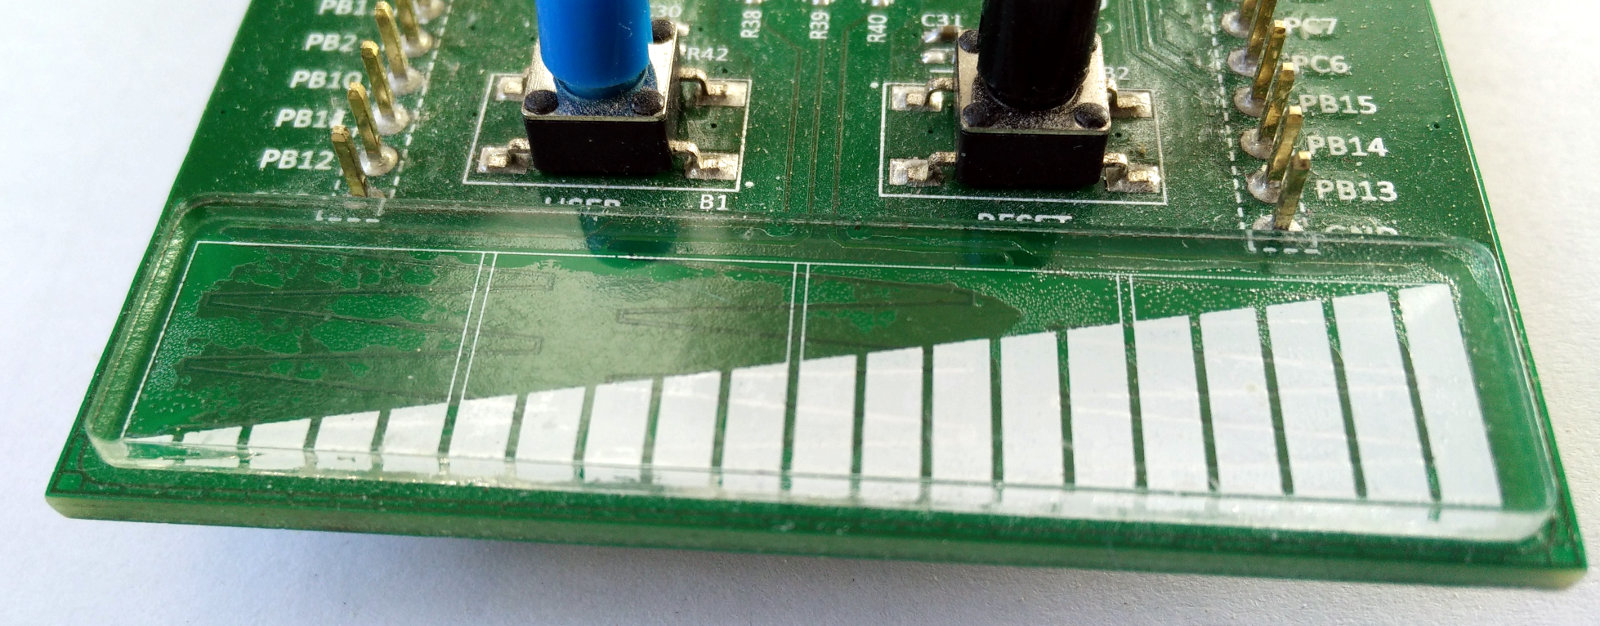
\includegraphics[width=0.5\textwidth] {img/disco-touch.jpg}
	\caption{\label{fig:disco-touch}The touch slider on a STM32F072 Discovery board}
\end{figure}

The principle of capacitive touch sensing using the \gls{TSC} is well explained in the microcontroller's reference manual~\cite{f072-rm}, the \gls{TSC} product training materials~\cite{stm-tsc-training, stm-tsc-ppt} and application notes from ST Microelectronics~\cite{stm-tsc-an1, stm-tsc-an2, stm-tsc-an3, stm-tsc-an4}. A key part of the \gls{TSC} is a set of analog switches which can be combined to form several different signal paths between external pins, Vdd, \gls{GND}, and an analog comparator. Two input pins are needed for every touch sensing channel: the sensing pad connects to one, the other is connected through a sampling capacitor  (47\,nF on the Discovery board) to \gls{GND}.

\begin{figure}[h]
	\centering
	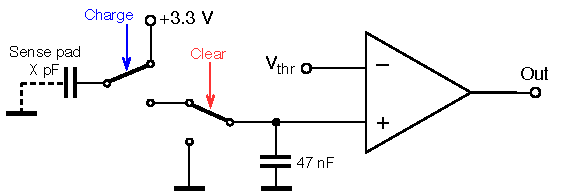
\includegraphics[scale=1] {img/tsc-function.pdf}
	\caption{\label{fig:tsc-schem}A simplified schematic of the touch sensing circuit}
\end{figure}

\noindent
Capacitive sensing is a sequential process described in the following steps:

\begin{enumerate}
	\item The sampling capacitor is discharged by connecting its free end to \gls{GND}.
	\item The sensing pad is connected to +3.3\,V and, acting as a capacitor, charged to this voltage. It stores a small amount of charge, depending on its capacitance---this is the variable property we are trying to measure.
	\item The free terminals of the two capacitors (the sensing pad and the sampling capacitor) are connected together and their voltages reach an equilibrium as a portion of the stored charge leaves the sensing pad and flows into the bigger capacitor.
	\item The steps (2) and (3) are repeated until the sampling capacitor's voltage exceeds a fixed threshold (set to a half of the supply voltage). The number of cycles needed to charge the sampling capacitor corresponds to the capacitance of the sensing pad.
\end{enumerate}

\noindent
A real voltage waveform measured on the sensing pad using an oscilloscope is shown in \cref{fig:tsc-wfm}.

\begin{figure}
	\centering
	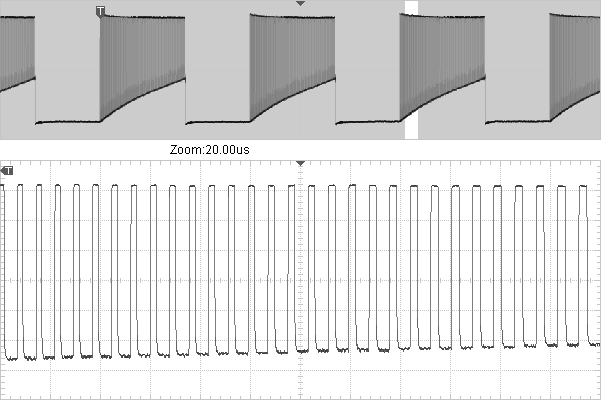
\includegraphics[width=.9\textwidth] {img/tsc-wfm-bw.png} \\
	\vspace{5mm}
	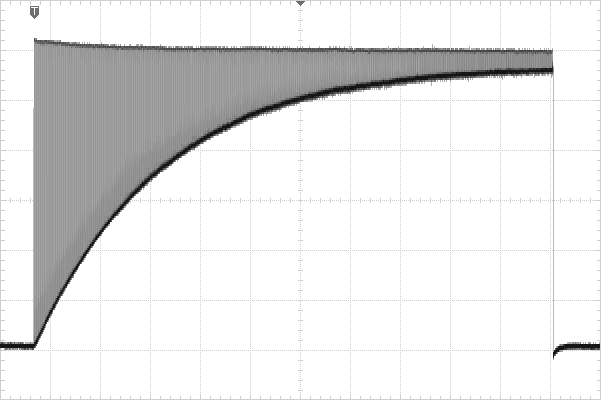
\includegraphics[width=.9\textwidth] {img/tsc-wfm2-bw.png}
	\caption[TSC operation oscilloscope screenshots]{\label{fig:tsc-wfm}A voltage waveform measured on the touch sensing pad. The bottom side of the envelope equals the sampling capacitor's voltage---this is the phase where both capacitors are connected. The detailed view (middle) shows the individual charging cycles. The bottom screenshot captures the entire waveform, left to continue until a timeout, after the analog comparator was disabled.}
\end{figure}




\part{Implementation}

\chapter{Application Structure}

GEX is designed to be modular and easy to extend. It is composed of a set of functional blocks (also called \textit{units}), sometimes available in more than one instance, which can be configured by the user to fit their application needs. The firmware is built around a \textit{core framework} which provides services to the functional blocks, such as a settings storage, resource allocation, message delivery and periodic updates.

In this chapter we will focus on the general function of the GEX module and will look at the services provided by the core framework. Individual functional blocks and the communication protocol will be described in \cref{sec:tinyframe,sec:units-overview}.

\iffalse
This and the following parts were written after implementing and evaluating the first hardware prototype and its firmware, therefore rather than describing the development process, it tends to talk about the completed solution and the decisions taken.
\fi

\section{User's View of GEX}

Before going into implementation details, we'll have a look at GEX from the outside, how the end user will see it. This should give the reader some context to better orient themselves in the following sections and chapters investigating the internal structure of the firmware and the communication protocol.

\begin{figure}[h]
	\centering
	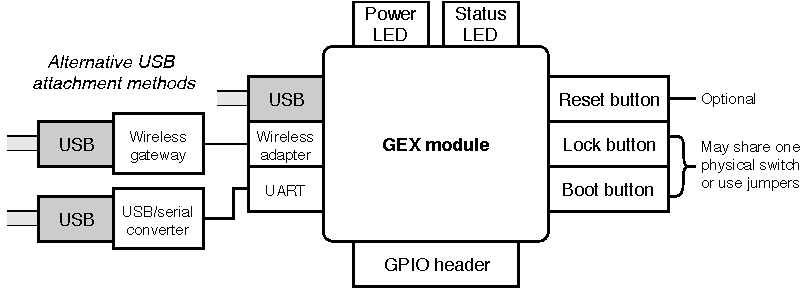
\includegraphics[scale=.95] {img/users-view.pdf}
	\caption{\label{fig:users-view-of-gex}Physical user interface of a GEX module}
\end{figure}

The GEX firmware can be flashed to a STM32 Nucleo or Discovery board or a custom \gls{PCB}. Discovery boards are equipped with a ``user \gls{USB}'' connector routed to the application \gls{MCU}; Nucleo boards have only the ST-Link \gls{USB} connector and, since the ST-Link version 2.1, offer a built-in USB-serial converter leading to one of the \gls{MCU}'s hardware \glspl{UART}.

After powering on, GEX loads its configuration from the Flash memory, configures its peripherals, sets up the function blocks and enables the selected communication interface(s). From this point, the module is operational and can be configured or used as needed by the user.

The physical user interface of the module is shown in \cref{fig:users-view-of-gex}. When a \gls{USB} cable connects the board to a \gls{PC}, the \gls{PC} \gls{OS} enumerates it and either recognizes the communication interface as \gls{CDCACM} (Virtual serial port), or leaves it without a software driver attached, to be accessed directly as raw \gls{USB} endpoints, based on GEX settings.
The connection using a physical UART and a USB/UART adapter works in a very similar way, as does the wireless connection (described in more detail below).

\subsection{Updating GEX Settings}

Two ways exist in which the module's settings can be modified: via the virtual Mass Storage disk, and through the control interface. We'll look at the file system method here; the API for a programmatic loading and updating of configuration will be explained in \cref{sec:tf-bulk-rw}.

The board is equipped with a button or a jumper labeled Lock. When the button is pressed or the jumper removed (or inserted, the polarity is configured in the firmware), the Mass Storage \gls{USB} interface is enabled. For the user, this means that a new disk will appear on their computer which they can open in a file manager. The disk provides a read/write access to configuration files.

The user edits a file as needed and saves it back to the disk. GEX processes the new content, tries to apply the changes and generates an updated version that includes any error messages or newly generated sections (when a new unit was registered). For the \gls{PC} \gls{OS} to recognize this change, the Mass Storage device momentarily reports that the media is unavailable to force the \gls{OS} to reload it. This is a similar mechanism to what happens when a memory card is removed from a reader. Now the user can reload the file in their editor, inspect the updated content and correct any possible mistakes. The settings, when applied successfully, should be immediately available to test using the communication interface. When everything is to the user's satisfaction, the updated settings are committed to the device's Flash memory by pressing the LOCK button again, or replacing the jumper.

\subsection{Connecting Using the Wireless Module}

In the case when a wireless module is installed on the \gls{PCB} and GEX is configured to use it, the radio link becomes a fallback connection when the \gls{USB} peripheral does not get enumerated within a short time after start-up.

To use it, the user needs to connect a wireless gateway module to their host \gls{PC} and use the radio link instead of a \gls{USB} cable. This connection works in a way similar to the hardware UART interface: it can be used to read and modify the configuration files and to access the functional blocks; the difference lies in a slightly different protocol required to communicate with the gateway itself, e.g. to pair it with the GEX module.

\subsection{Using the Control Interface}

Now that GEX is connected and configured, the user can start using it. This involves writing a program in C or Python that uses the GEX client library, using the Python library from MATLAB, or controlling GEX using a \gls{GUI} front-end built on those libraries. The configuration can be stored in the module, but it is also possible to temporarily replace it using the control \gls{API}. This way, the settings are loaded automatically when the user's program starts and may differ for different programs.

\section{Internal Structure Block Diagram}

The data flows and other internal logic of the firmware are depicted in \cref{fig:gex-internal}, with more explanation following in this chapter. The interchangeable role of the three communication interfaces can be clearly seen in the diagram, as well as the central role of the message queue which decouples interrupts from the processing thread.

\begin{figure}[h]
	\centering
	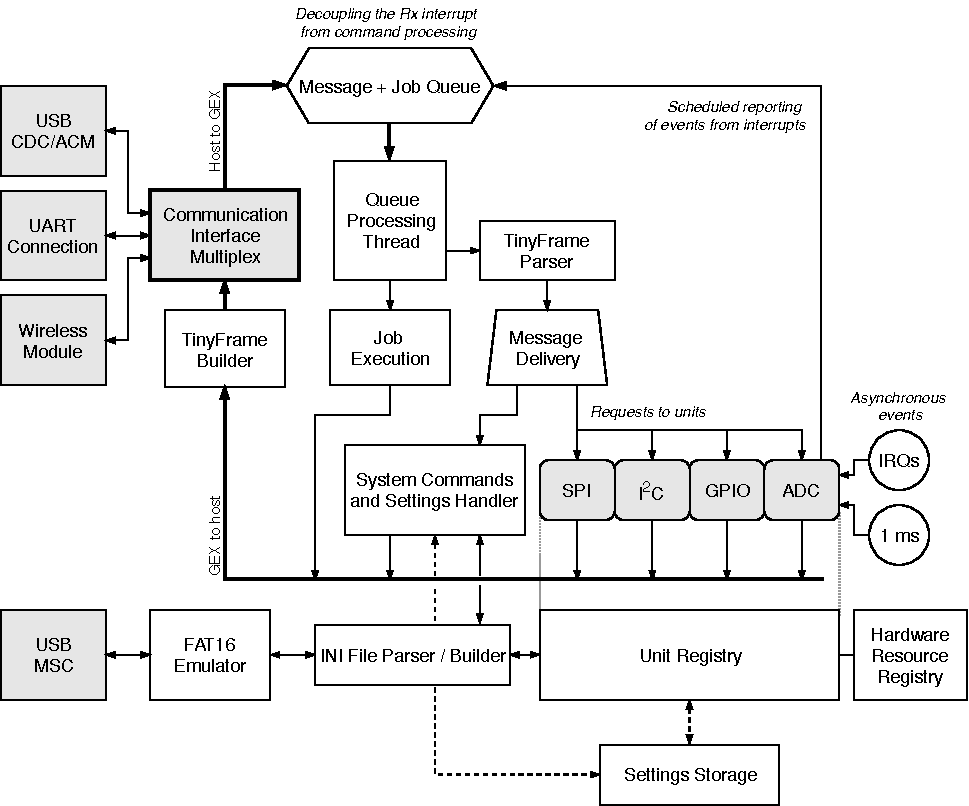
\includegraphics[scale=1] {img/gex-internal.pdf}
	\caption{\label{fig:gex-internal}Block diagram showing the internal logic in the GEX firmware}
\end{figure}

\section{FreeRTOS Synchronization Objects Usage}

The firmware is built on FreeRTOS (\cref{sec:freertos}) and a number of its synchronization objects and patterns are used to make its operation more robust.

\subsection{Message and Job Queue}

The message and job queue, seen in \cref{fig:gex-internal}, is used to decouple asynchronous interrupts from message transmission. All three communication interfaces use interrupts for the asynchronous handling of incoming messages. The same interrupt handler receives an event after a transmission was completed. The queue ensures that messages can be received during the transmission of a large response that demands the use of multiple transmissions.

The ``transmission complete'' interrupt signals this fact to the message processing task using a binary semaphore. The semaphore is released in the interrupt and take before a new block of data is transmitted. If more data needs to be transmitted, the queue task waits on the semaphore and enters a Blocked state until the semaphore becomes available again.

Two mutexes are used in the firmware: one that guards access to TinyFrame until the previous message was fully transmitted, and one to guard a shared memory buffer used, among other, by unit drivers during the serialization and parsing of a configuration file. The hardware resource registry (explained in \cref{sec:res-allocation}) does not need mutexes for individual resources, as a concurrent access to those fields can never happen thanks to the way the system is organized.

\section{Functional Blocks} \label{sec:units-function}

GEX's user-facing functions are implemented in \textit{unit drivers}. Those are mutually independent modules in the firmware that the user can enable and configure using a configuration file. There can be multiple instances of each unit type. However, we are limited by hardware constraints: e.g., there may be only one \gls{ADC} peripheral, two \gls{SPI} ports and so on. The assignment of those hardware resources to units is handled by the \textit{resource registry} (\cref{sec:res-allocation}).

Each unit is defined by a section in the configuration file \verb|UNITS.INI|. It is given a name and a \textit{callsign}, which is a number that serves as an address for message delivery. A unit is internally represented by a data object with the following structure:

\begin{itemize}
	\item Name
	\item Callsign (one byte)
	\item Configuration parameters loaded from the unit settings
	\item State variables updated at run-time by user commands or internal functions
	\item A reference to the unit driver
\end{itemize}

The unit driver handles commands sent from the host \gls{PC}, initializes and de-initializes the unit based on its settings, and implements other aspects of the unit's function, such as periodic updates and interrupt handling. Unit drivers may expose public \gls{API} functions to make it possible to control the unit from a different driver, allowing the creation of ``macro units''.

\section{Source Code Layout}

\begin{wrapfigure}[22]{r}{0.4\textwidth}
	\scriptsize\vspace{-3em}
	\begin{verbatim}
	├── build
	│   ├── firmware.bin
	│   └── firmware.dfu
	├── Drivers
	│   ├── CMSIS
	│   │   └── Device / ST / STM32F0xx
	│   └── STM32F0xx_HAL_Driver
	├── Middlewares / Third_Party / FreeRTOS
	├── Src
	│   └── main.c
	├── User
	│   ├── USB / STM32_USB_Device_Library
	│   │   ├── Class
	│   │   │   ├── CDC
	│   │   │   ├── MSC
	│   │   │   └── MSC_CDC
	│   │   └── Core
	│   ├── platform
	│   │   ├── plat_compat.h
	│   │   └── platform.c
	│   ├── units
	│   │   ├── adc
	│   │   ├── digital_out
	│   │   ...
	│   ├── FreeRTOSConfig.h
	│   └── gex.mk
	└── Makefile
	\end{verbatim}
	\vspace{-1em}
	\caption{\label{fig:repo-structure} The general structure of the source code repository}
\end{wrapfigure}

Looking at the source code repository (\cref{fig:repo-structure}), at the root we'll find the device specific driver libraries and support files provided by ST Microelectronics, the FreeRTOS middleware, and a folder called \verb|User| containing the GEX application code. This division is useful when porting the firmware to a different microcontroller, as the GEX folder is mostly platform-independent and can be simply copied (of course, adjustments are needed to accompany different hardware peripheral versions etc.). The GEX core framework consists of everything in the \verb|User| folder, excluding the \verb|units| directory in which the individual units are implemented. Each unit driver must be registered in the file \verb|platform.c| to be available for the user to select. The file \verb|plat_compat.c| includes platform-specific headers and defines e.g. which pin to use for a status \gls{LED} or the LOCK button.

The \gls{USB} Device library, which had to be modified to support a composite class, is stored inside the \verb|User| folder too, as it is compatible with all STM32 microcontrollers that support \gls{USB}.


\section{Functions of the Core Framework}

The core framework forms the skeleton of the firmware and usually doesn't need any changes when new user-facing features are added. It provides the following services:

\begin{itemize}
	\item Hardware resource allocation (\cref{sec:res-allocation})
	\item Settings storage and loading (\cref{sec:settings-storage})
	\item Functional block (\textit{units}) initialization (\cref{sec:units-function})
	\item The communication port with different back-ends: \gls{USB}, \gls{UART}, wireless (\cref{sec:com-ports})
	\item Message sending and delivery (\cref{sec:message_passing})
	\item Interrupt management and routing to functional blocks (\cref{sec:irq-routing})
	\item Virtual mass storage for configuration files (explained in \cref{sec:fat16})
\end{itemize}

When the firmware needs to be ported to a different STM32 microcontroller, the core framework is relatively straightforward to adapt and the whole process can be accomplished in a few hours. The time consuming part is modifying the functional blocks to work correctly with the new device's hardware.


\subsection{Resource Allocation} \label{sec:res-allocation}

\begin{figure}[h]
	\centering
	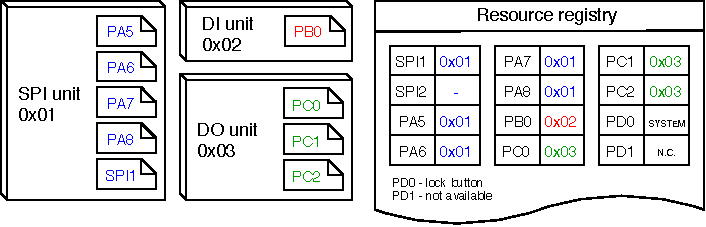
\includegraphics[scale=1] {img/resource-repository.pdf}
	\caption{\label{fig:resource-repository}An example allocation in the resource registry}
\end{figure}

The microcontroller provides a number of hardware resources that require exclusive access: GPIO pins, peripheral blocks (\gls{SPI}, \gls{I2C}, \gls{UART}\textellipsis), \gls{DMA} channels. If two units tried to control the same pin, the results would be unpredictable; similarly, with a multiple access to a serial port, the output would be a mix of the data streams and completely useless.

To prevent a multiple access, the firmware includes a \textit{resource registry} (\cref{fig:resource-repository}). Each individual resource is represented by a field in a resource table together with its owner's callsign. Initially all resources are free, except for those not available on the particular platform (i.e. a GPIO pin PD1 may be disabled if not present on the microcontroller's package).

The resources used by the core framework are taken by a virtual unit \verb|SYSTEM| on start-up to prevent conflicts with the user's units. This is the case of the status \gls{LED}, the LOCK button, \gls{USB} pins, the communication \gls{UART}, the pins and an \gls{SPI} peripheral connecting the wireless module, pins used for the crystal oscillator, and the timer/counter which provides the system timebase.


\subsection{Settings Storage} \label{sec:settings-storage}

\begin{figure}[h]
	\centering
	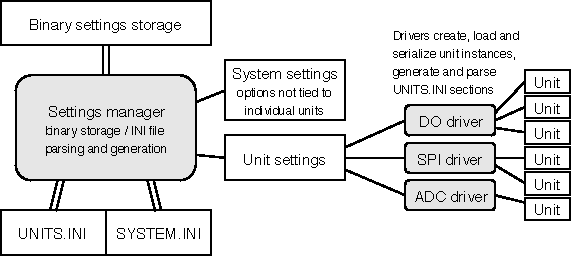
\includegraphics[scale=1] {img/settings-storage.pdf}
	\caption{\label{fig:settings-storage}Structure of the settings subsystem}
\end{figure}

The system and unit settings are written, in a binary form, into designated pages of the microcontroller's Flash memory. The unit settings serialization and parsing is implemented by the respective unit drivers.

As the settings persist after a firmware update, it is important to maintain backwards compatibility. This is achieved by prefixing the settings block of each unit with a version number. When the settings are loaded by a new version of the firmware, it first checks the version and decides whether to use the old or new format. When the settings are next changed, the new format will be used.

The INI files, which can be edited through the communication \gls{API} or using a text editor with the virtual mass storage, are parsed and generated on demand and are never stored in the Flash or \gls{RAM}, other than in short temporary buffers. The INI parser processes the byte stream on-the-fly as it is received, and a similar method is used to build a INI file from the configured units and system settings.

\subsection{Communication Ports} \label{sec:com-ports}

The firmware supports three different communication ports: hardware \gls{UART}, \gls{USB} (virtual serial port), and a wireless connection. Each interface is configured and accessed in a different way, but for the rest of the firmware (and for the \gls{PC}-side application) they all appear as a full duplex serial port. To use interfaces other than \gls{USB}, the user must configure those in the system settings (a file \verb|SYSTEM.INI| on the configuration disk).

At start-up, the firmware enables the \gls{USB} peripheral, configures the device library and waits for enumeration by the host \gls{PC}. When not enumerated, it concludes the \gls{USB} cable is not connected, and tries some other interface. The \gls{UART} interface cannot be tested as reliably, but it is possible to measure the voltage on the Rx pin. When idle, a \gls{UART} Rx line should be high (here 3.3\,V). The wireless module, when connected using \gls{SPI}, can be detected by reading a register with a known value and comparing those.

\subsubsection{USB Connection}

GEX uses vid:pid \verb|1209:4c60| and the wireless gateway \verb|1209:4c61|. The \gls{USB} interface uses the \gls{CDCACM} \gls{USB} class (\cref{sec:cdc-acm}) and consists of two bulk endpoints with a payload size of up to 64 bytes.

\subsubsection{Communication UART}

The parameters of the communication \gls{UART} (such as the baud rate) are defined in \verb|SYSTEM.INI|. It is mapped to pins PA2 and PA3; this is useful with STM32 Nucleo boards that do not include a User \gls{USB} connector, but provide a \gls{USB}-serial bridge using the on-board ST-Link programmer, connected to those pins.

This is identical to the \gls{USB} connection from the \gls{PC} application's side, except a physical \gls{UART} is necessarily slower and does not natively support flow control. The use of the Xon and Xoff software flow control is not practical with binary messages that could include those bytes by accident, and the ST-Link \gls{USB}-serial adapter does not implement hadware flow control.

\subsubsection{Wireless Connection}

The wireless connection uses an on-board communication module and a separate device, a wireless gateway, that connects to the \gls{PC}. The wireless gateway is interfaced differently from the GEX board itself, but it also shows as a virtual serial port on the host \gls{PC}. This is required to allow communicating with the gateway itself through the \gls{CDCACM} interface in addition to addressing the end devices.

This interface will be explained in more detail in \cref{sec:wireless}.

\subsection{Message Passing} \label{sec:message_passing}

One of the key functions of the core framework is to deliver messages from the host \gls{PC} to the right units. This functionality resides above the framing protocol, which will be described in \cref{sec:tinyframe}.

A message that is not a response in a multi-part session (this is handled by the framing library) is identified by its Type field. Two main groups of messages exist: \textit{system messages} and \textit{unit messages}. System messages can access the INI files, query a list of the available units, restart the module etc. Unit messages are addressed to a particular unit by their callsign (see \cref{sec:units-function}), and their payload format is defined by the unit driver. The framework reads the message type, then the callsign byte, and tries to find a matching unit in the unit list. If no unit with the callsign is found, an error response is sent back, otherwise the unit driver is given the message to handle it as required.

The framework provides one more messaging service to the units: event reporting. An asynchronous event, such as an external interrupt, an \gls{ADC} trigger or an \gls{UART} data reception needs to be reported to the host. This message is annotated by the unit callsign so the user application knows its origin.


\subsection{Interrupt Routing} \label{sec:irq-routing}

Interrupts are an important part of almost any embedded application. They provide a way to rapidly react to asynchronous external or internal events, temporarily leaving the main program, jumping to an interrupt handler routine, and then returning back after the event is handled. Interrupts are also the way FreeRTOS implements multitasking without a multi-core processor.

In the Cortex-M0-based STM32F072, used in the initial GEX prototypes, the interrupt handlers table, defining which routine is called for which interrupt, is stored in the program memory and cannot be changed at run-time. This is a complication for the modular structure of GEX where different unit drivers may use the same peripheral, and we would want to dynamically assign the interrupt handlers based on the active configuration. Let's have a look at an interrupt handler, in this case handling four different \gls{DMA} channels, as is common in STM32 microcontrollers:

\begin{minted}{c}
void DMA1_Channel4_5_6_7_IRQHandler(void)
{
    if (LL_DMA_IsActiveFlag_GI4(DMA1)) { /* handle DMA1 channel 4 */ }
    if (LL_DMA_IsActiveFlag_GI5(DMA1)) { /* handle DMA1 channel 5 */ }
    if (LL_DMA_IsActiveFlag_GI6(DMA1)) { /* handle DMA1 channel 6 */ }
    if (LL_DMA_IsActiveFlag_GI7(DMA1)) { /* handle DMA1 channel 7 */ }
}
\end{minted}

It is evident that multiple units might need to use the same interrupt handler, even at the same time, since each \gls{DMA} channel is configured, and works, independently. GEX implements a redirection scheme to accomplish such interrupt sharing: All interrupt handlers are defined in one place, accompanied by a table of function pointers. When a unit driver wants to register an interrupt handler, it stores a pointer to it in this redirection table. Then, once an interrupt is invoked, the common handler checks the corresponding entry in the table and calls the referenced routine, if any. Conversely, when a unit driver deinitializes a unit, it removes all interrupt handlers it used, freeing the redirection table slots for other use.












\chapter{Communication Protocol} \label{sec:tinyframe}

GEX can be controlled through a hardware \gls{UART}, the \gls{USB}, or over a wireless link. To minimize the firmware complexity, all the three connection methods use the same binary messaging protocol and are functionally interchangeable.

\begin{wrapfigure}[9]{r}{0.38\textwidth}
	\vspace{-1em}
	\centering
	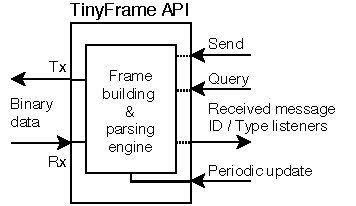
\includegraphics[scale=1]{img/tf-conceptual.pdf}
	\caption{\label{fig:tf_conceptual}TinyFrame API}
\end{wrapfigure}

GEX uses the \textit{TinyFrame}~\cite{tinyframerepo} framing library, developed, likewise, by the author, but kept as a separate project for easier re-use in different applications. The library implements frame building and parsing, including checksum calculation, and provides high-level \gls{API}.

Both peers, GEX and the client library running on the host \gls{PC}, are at an equal level: either side can independently send a message at any time. The communication is organized in transactions; a transaction consists of one or more messages going in either direction. A message can be stand-alone, or chained to another, typically a request, using the frame ID field; this is the major advantage over text-based protocols, like AT commands, where all messages are independent and their relation to each other is not always clear.

\section{Binary Payload Structure Notation}

Binary payloads are described in several places of this text. We use a shortened notation derived from the C language to represent field data types:

\begin{pldlist}
	\cfield{bool} -- 8-bit field allowing values 0 (false) and 1 (true)
	\cfield{u8}, \cfieldx{u16}, \cfieldx{u32}  -- unsigned 8-, 16-, or 32-bit integer
	\cfield{i8}, \cfieldx{i16}, \cfieldx{i32}  -- signed (two's complement) 8-, 16-, or 32-bit integer
	\cfield{char} -- an 8-bit ASCII character
	\cfield{float} -- single-precision (32-bit) IEEE~754~\cite{floatpaper} floating point number
	\cfield{double} -- double-precision (64-bit) IEEE~754~\cite{floatpaper} floating point number
	\cfield{u8[]} -- array of variable length
	\cfield{u8[n]} -- array of length n
	\cfield{cstring} -- zero-terminated character string (like \cfieldx{char[]}, ending with a 0x00 byte)
\end{pldlist}


\section{Frame Structure}

Message frames have the following structure (all little-endian):

\begin{boxedpayload}[``TinyFrame'' frame structure, as used in GEX]
	\cfield{0x01} start-of-frame marker
	\cfield{u16} frame ID
	\cfield{u16} payload length
	\cfield{u8} frame type
	\cfield{u8} header checksum
	\cfield{u8[]} payload
	\cfield{u8} payload checksum (omitted for empty payloads)
\end{boxedpayload}

\iffalse
\begin{table}[h]
	\centering
	%\hspace{-1.5em}
	\begin{tabular}{rccccccc}
		\toprule
		\multicolumn{1}{c|}{} &
		\multicolumn{5}{c}{Header}&
		\multicolumn{2}{|c}{Body} \\
		\midrule
		%
		\textit{Field} &
			\textbf{SOF} &
			\textbf{Frame ID} &
			\makecell{ \Gape{\textbf{Payload}} \\ \Gape{\textbf{Length}} } &
			\makecell{ \textbf{Frame} \\ \textbf{type} } &
			\makecell{ \textbf{Header} \\ \textbf{checksum} } &
			\textbf{Payload} &
			\makecell{ \textbf{Payload} \\ \textbf{checksum} } \\
		%
		\midrule
		\textit{Bytes} &
			 1  &
			 2  &
			 2  &
			 1  &
			 1  &
			 ... &
			 1 \\
		%
		\bottomrule
	\end{tabular}
\end{table}
\fi

\textit{Frame ID}, which could be better described as \textit{Transaction ID}, uniquely identifies each transaction. The most significant bit is set to a different value in each peer to avoid ID conflicts, and the rest of the ID field is incremented with each initiated transaction.

\section{Message Listeners} \label{sec:tf_listeners}

After sending a message that should receive a response, the peer registers an \textit{ID listener} with the ID of the sent message. A response reuses the original frame ID and when it is received, this listener is called to process it. ID listeners can also be used to receive multi-part messages re-using the original ID.

\textit{Frame type} describes the payload and does not have any prescribed format in TinyFrame; its values are defined by the application. A \textit{type listener} may be registered to handle all incoming messages with a given frame type. It works in a similar way to an ID listener, but has a lower priority.

Each message can be handled by only one listener, unless the listener explicitly requests it to be passed on. Messages not handled by any listener are given to a default listener, which can, e.g., write an error to a debug log.

\section{Designated Frame Types}

\Cref{fig:tf_types} lists the frame types defined by GEX. It is divided into four logical sections: General, Bulk Read/Write, Unit Access, and Settings. The payloads belonging to those frame types will be outlined in the following sections.

\begin{table}[h]
	\centering
	\begin{tabular}{clll}
		\toprule
		\textbf{Frame type} & \textbf{Function} & \textbf{Note} \\
		\midrule
		0x00 & Success & \textit{Payload depends on context} \\
		0x01 & Ping & \textit{GEX responds with Success and its version string} \\
		0x02 & Error & \textit{Payload contains the error message} \\
		\midrule
		0x03 & Bulk Read Offer & \textit{An offer of data to read using }0x04 \\
		0x04 & Bulk Read Poll & \textit{Requesting to read a block of data} \\
		0x05 & Bulk Write Offer & \textit{An offer to receive a bulk write transaction} \\
		0x06 & Bulk Data & \textit{Used for both reading and writing} \\
		0x07 & Bulk End & \textit{Marks the last ``Bulk Data'' frame} \\
		0x08 & Bulk Abort & \textit{} \\
		\midrule
		0x10 & Unit Request & \textit{Request to a unit} \\
		0x11 & Unit Report & \textit{Spontaneous event generated by a unit} \\
		\midrule
		0x20 & List Units & \textit{Read a list of all instantiated units} \\
		0x21 & INI Read & \textit{Request a bulk read transaction of an INI file} \\
		0x22 & INI Write & \textit{Request a bulk write transaction of an INI file} \\
		0x23 & Persist Config & \textit{Write updated configuration to flash} \\
		\bottomrule
	\end{tabular}
\caption{\label{fig:tf_types}Frame types used by GEX}
\end{table}


\section{Bulk Read and Write Transactions} \label{sec:tf_bulk_rw}

The bulk read and write transactions are generic, multi-message exchanges which are used to transfer the INI configuration files. They could additionally be used by some future unit requiring to transfer a large amount of data (e.g., to read image data from a camera).

The reason for splitting a long file into multiple messages, rather than sending it all in one, lies in the hardware limitations of the platform, specifically its small amount of \gls{RAM} (the STM32F072 has only 16\,kB). A message cannot be processed until its payload checksum is received and verified; however, the configuration file can have several kilobytes, owning to the numerous explanatory comments, which would require a prohibitively large data buffer. The chunked transaction could, additionally, be extended to support message re-transmission on timeout without sending the entire file again.

A read or write transaction can be aborted by a frame \CmdBulkAbort at any time, though aborting a write transaction may leave the configuration in a corrupted state. As hinted in the introduction of this chapter, a transaction is defined by sharing a common frame ID. Thus, all frames in a bulk transaction must have the same ID, otherwise the ID listeners would not be called for the subsequent messages.

\Cref{fig:bulk_rw} shows a diagram of the bulk read and write data flow.

\begin{figure}
	\centering
	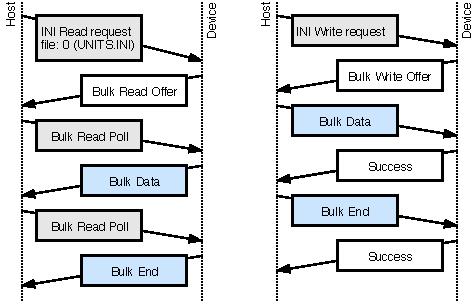
\includegraphics[scale=1.5]{img/bulk-read-write.pdf}
	\caption{\label{fig:bulk_rw}A diagram of the bulk read and write transaction.}
\end{figure}

\subsection{Bulk Read}

To read an INI file, we first send a frame \CmdINIRead, specifying the target file in the payload:

\begin{boxedpayload}[Frame \CmdINIRead payload structure]
	\cfield{u8} which file to write
		\begin{pldlist}
			\item 0 \dots UNITS.INI
			\item 1 \dots SYSTEM.INI
		\end{pldlist}
\end{boxedpayload}

What follows is a standard bulk read transaction with the requested file.
GEX offers the file for reading with a frame \CmdBulkReadOffer:

\begin{boxedpayload}[Frame \CmdBulkReadOffer payload structure]
	\cfield{u32} full size of the file in bytes
	\cfield{u32} largest chunk that can be read at once
\end{boxedpayload}

Now we can proceed to read the file using \CmdBulkReadPoll, which is always responded to with \CmdBulkData, or \CmdBulkEnd if this was the last frame. Data frames have only the useful data as their payload. The \CmdBulkReadPoll payload specifies how many bytes we want to read:

\begin{boxedpayload}[Frame \CmdBulkReadPoll payload structure]
	\cfield{u32} how many bytes to read (at most)
\end{boxedpayload}

\begin{boxedpayload}[Frame \CmdBulkData or \CmdBulkEnd payload in a ``read'' transaction]
\cfield{char[]} a chunk of the read file
\end{boxedpayload}

\subsection{Bulk Write}

To overwrite an INI file, we first send a frame \CmdINIWrite with the file size as its payload. The name of the file is irrelevant, as it is detected automatically by inspecting the content.

\begin{boxedpayload}[Frame \CmdINIWrite payload structure]
	\cfield{u32} size of the written file, in bytes
\end{boxedpayload}

\noindent
The write request is confirmed by a frame \CmdBulkWriteOffer sent back:

\begin{boxedpayload}[Frame \CmdBulkWriteOffer payload structure]
	\cfield{u32} total bytes to write (here copied from the request frame)
	\cfield{u32} how many bytes may be written per message
\end{boxedpayload}

We can now send the file as a series of frames of type \CmdBulkData, or \CmdBulkEnd in the last frame, with chunks of the data as their payloads. Each frame is confirmed by \CmdSuccess.

\begin{boxedpayload}[Frame \CmdBulkData or \CmdBulkEnd payload in a ``write'' transaction]
	\cfield{char[]} a chunk of the written file
\end{boxedpayload}

\subsection{Persisting the Changed Configuration to Flash}

The written INI file is immediately parsed and the settings are applied. However, these changes are not persistent: they exist only in \gls{RAM} and will be lost when the module restarts. To save the current state to Flash, issue a frame \CmdPersistConfig. This has the same effect as closing the virtual mass storage by pushing the Lock button.

\iffalse
It should be noted that after flashing a firmware, the Flash control registers may remain in an unexpected state and the module must first be manually restarted before attempting to persist settings. Otherwise an assertion will fail and the module is restarted by a watchdog, losing the temporary changes.
% TODO there must be a workaround, and then this paragraph can be removed.
\fi


\section{Reading the List of Units}

The frame \CmdListUnits requests a list of all available units in the GEX module. The list includes all units' callsigns, names and types. The response payload has the following format:

\begin{boxedpayload}[Frame \CmdListUnits response structure]
	\cfield{u8} the number of available units
	\item For each unit:
		\begin{pldlist}
			\cfield{u8} unit callsign
			\cfield{cstring} unit name
			\cfield{cstring} unit type
		\end{pldlist}
\end{boxedpayload}


\section{Unit Requests and Reports} \label{sec:unit_requests_reports}

Frame types \CmdUnitRequest and \CmdUnitReport are dedicated to messages sent to and by unit instances. Each has a fixed header (\textit{inside the payload}) followed by unit-specific data.

\subsection{Unit Requests}\label{sec:unit_requests_format}

Unit requests deliver a message from the host to a unit instance. Unit drivers implements different commands, each with its own payload structure. The frame \CmdUnitRequest has the following structure:

\begin{boxedpayload}[Frame \CmdUnitRequest payload structure]
	\cfield{u8} unit callsign
	\cfield{u8} command number, handled by the unit driver
	\cfield{u8[]} command payload, handled by the unit driver; its size and content depend on the unit driver and the particular command number, as defined in \cref{sec:units_overview}
\end{boxedpayload}

The most significant bit of the command byte (0x80) has a special meaning: when set, the message delivering routine responds with \CmdSuccess after the command completes, unless an error occurred. That is used to get a confirmation that the message was delivered and the module operates correctly (as opposed to, e.g., a lock-up resulting in a watchdog reset). Requests which normally generate a response (e.g., reading a value from the unit) should not be sent with this flag, as that would produce two responses at once.

\subsection{Unit Reports}\label{sec:unit_reports_format}

Several unit types can produce asynchronous events, such as reporting a pin change, or a triggering condition. The event is timestamped and sent with a frame type \CmdUnitReport:

\begin{boxedpayload}[Frame \CmdUnitReport payload structure]
	\cfield{u8} unit callsign
	\cfield{u8} report type, defined by the unit driver
	\cfield{u64} event time (microseconds since power-on)
	\cfield{u8[]} report payload; similar to requests, the payload structure depends on the unit driver and the particular report type, as defined in \cref{sec:units_overview}
\end{boxedpayload}


















\chapter{Wireless Interface} \label{sec:wireless}

Four methods of a wireless connection have been considered: Bluetooth (e.g. with CC2541), WiFi with ESP8266, a 868\,MHz long range link with SX1276, and a 2.4\,GHz link with nRF24L01+. Bluetooth was dismissed early for its complexity, and ESP8266 for its high consumption in continuous reception mode, although both solutions might be viable for certain applications and with more development time.

The Semtech SX1276~\cite{semtech-manual} and Nordic Semiconductor nRF24L01+ ~\cite{nrf-manual} transceivers have both been tested using the first GEX prototype, proving its usefulness as a hardware development tool, and it has been confirmed they could fulfill the requirements of our application.

\begin{figure}[h]
	\centering
	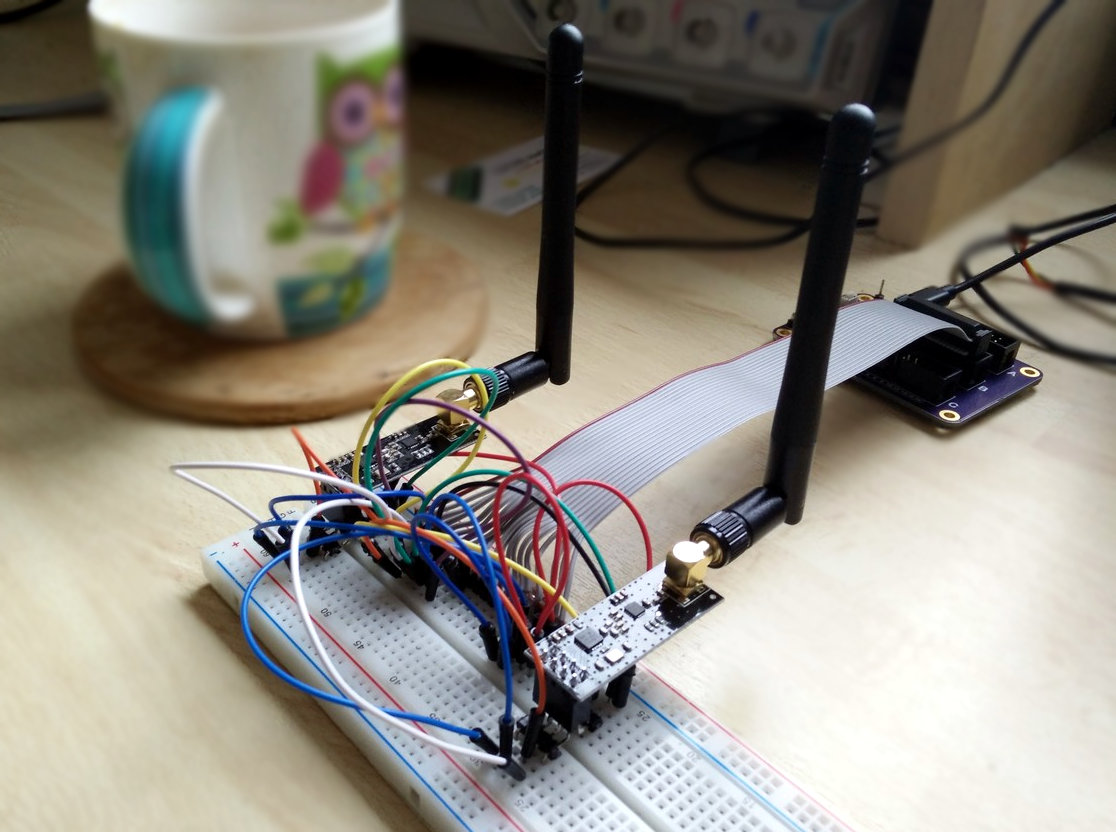
\includegraphics[width=.7\textwidth]{img/nrf-testing.jpg}
	\caption{Test setup with a GEX prototype controlling two nRF24L01+ modules}
\end{figure}

\section{Modulations Overview}

A brief overview of the different signal modulation techniques is presented here to aid the reader with understanding of table~\ref{fig:nrf-sx-comparison} and the rest of the chapter.

\subsection{On-Off Keying (OOK)}

In \gls{OOK}, the carrier generator is switched on and off to transmit ones and zeros.

\subsection{Frequency Shift Keying (FSK)}

\Gls{FSK} uses a change of the carrier frequency to transmit data. The simplest form of \gls{FSK} is \gls{BFSK}, which uses a pair of alternating frequencies to transmit ones and zeros.

\subsection{Gaussian Frequency Shift Keying (GFSK)}

\Gls{GFSK} is an improvement over basic \gls{FSK} which does not switch between the different frequencies instantaneously, but uses a Gaussian filter to make the changes less abrupt, which reduces the side-band interference otherwise generated by the sharp edges. This scheme can be imagined as sending the binary waveform through a Gaussian filter and then modulating a \gls{VCO} with its output, rather than changing the \gls{VCO}'s control voltage discretely. \Gls{GFSK} is used in the Bluetooth standard.

\subsection{Minimum-Shift Keying (MSK)}

\Gls{MSK} is another \gls{FSK}-based modulation scheme. In \gls{MSK}, the frequencies representing different symbols are chosen such that there are no sharp changes in the phase of the output waveform, the modulation is \textit{phase-coherent}. This is another way to reduce side-band interference.

\subsection{Gaussian Minimum-Shift Keying (GMSK)}

\Gls{GMSK} is a variant of \gls{MSK} which uses a Gaussian filter to shape the digital signal before sending it to the oscillator. The principle is similar to \gls{GFSK}, and it is a yet another way to reduce side-band interference and increase spectral efficiency. \gls{GMSK} is used in the \gls{GSM}.

\subsection{LoRa Modulation}

LoRa is a patented proprietary modulation developed by Semtech. It uses a direct sequence frequency hopping spread spectrum modulation and can achieve very long range transmission (over 10\,km is not uncommon). LoRa is available only with transceiver \glspl{IC} produced by Semtech and for this reason it is rather expensive.

\section{Comparing SX1276 and nRF24L01+}

The two transceivers are compared in table~\ref{fig:nrf-sx-comparison}. It is apparent that each of them has its strengths and weaknesses, which will be discussed below.

\begin{table}[h]
	\centering
	\begin{tabulary}{\textwidth}{lLL}
		\toprule
		\textbf{Parameter} & \textbf{SX1276} & \textbf{nRF24L01+} \\
		\midrule
		\textbf{Connection} & SPI (4 pins) + up to 6 IRQ & SPI (4 pins), CE, IRQ \\
		\textbf{Frequency band} & 868\,MHz or 433\,MHz & 2.4\,GHz \\
		\textbf{Data rate} & up to 300\,kbps & 250--2000\,kbps \\
		\textbf{Modulation} & (G)FSK, (G)MSK, OOK, LoRa & GFSK \\
		%		\textbf{Bandwidth} & 7--500\,kHz per channel & 0.7--2\,MHz per channel \\
		\textbf{Range (est.)} & over 10\,km & up to 1\,km \\
		\textbf{Consumption Rx} & 10.8--12\,mA & 12.6--13.5\,mA \\
		\textbf{Consumption Tx} & 20--120\,mA & 7--11.3\,mA \\
		\textbf{Idle power (max)} & 1\,$\mu$A sleep, 2\,mA stand-by & 0.9\,$\mu$A sleep, 320\,$\mu$A stand-by \\
		\textbf{Max packet size} & 300 bytes & 32 bytes \\
		\textbf{Reset} & NRESET pin & Vdd disconnect \\
		\textbf{Extra} & LoRa FHSS, packet engine & ShockBurst protocol engine \\
		\textbf{Price} & \$7.3 & \$1.6 \\
		\bottomrule
	\end{tabulary}
	\caption[Comparison of the SX1276 and nRF24L01+ wireless transceivers]{\label{fig:nrf-sx-comparison}Comparison of the SX1276 and nRF24L01+ wireless transceivers, using data from their datasheets (price in USD from DigiKey in a 10\,pcs. quantity, recorded on May 6th 2018)}
\end{table}

SX1276 supports additional modulation modes, including a proprietary LoRa scheme with a frequency-hopping spread spectrum modulation that can be received at a distance up to 20\,km in ideal conditions. The long-range capability is reflected in a higher consumption during transmission. However, its consumption in receiver mode is slightly lower than that of the nRF24L01+.

nRF24L01+ provides higher data rates at short distances. Its power consumption is comparable or lower than that of the SX1276. It lacks a dedicated reset pin, but that can be easily worked around using an external transistor to momentarily disconnect its Vdd pin.

Both devices implement some form of a packet engine with error checking; that of the nRF24L01+, called ShockBurst, is more advanced as it implements acknowledgment responses and automatic re-transmission, leading to a potentially more robust communication without an additional overhead on the side of the microcontroller.


\section{Integration of the nRF24L01+ into GEX}

The nRF24L01+ was selected to be integrated into GEX thanks to its inclusion of the ShockBurst engine, higher possible data rates and significantly lower price. The SX1276, nonetheless, remains an interesting option that could be used as an alternative in the future, should the need for a long range communication arise.

A separate device, the \textit{GEX wireless gateway}, was developed to provide the PC connection to a nRF24L01+ module. It is based on the STM32F103 microcontroller in its smallest package (LQFP48), selected for its low cost and good availability.

\todo[inline]{more about the hardware}

\subsection{The Wireless Gateway Protocol}

\begin{wrapfigure}[17]{r}{0.38\textwidth}
	\vspace{-1em}
	\centering
	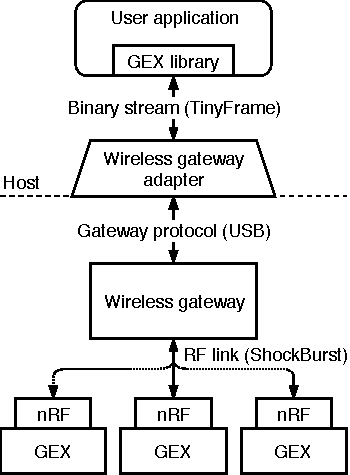
\includegraphics[scale=0.9]{img/rf-gw.pdf}
	\caption{A block diagram of the wireless connection}
\end{wrapfigure}

The gateway presents itself to the host as a \gls{CDCACM} device, much like the GEX modules themselves (here called \textit{nodes}) when connected over \gls{USB}. It implements a simple protocol which encapsulates the binary data sent to or from a connected node. The wrapped GEX protocol, which is described in chapter~\ref{sec:tinyframe}, remains unchanged.

The gateway has a 4-byte network ID, a number derived from the \gls{MCU}'s unique ID by calculating its 32-bit \gls{CRC}. The network ID must be entered into all nodes that wish to communicate with the gateway. Additionally, each module is assigned a 1-byte number which serves as its address in the network. The gateway can receive messages from up to 6 nodes.

All messages sent to or from the gateway are a multiple of 64 bytes long, padded with zeros if shorter. The message starts with a control byte determining its type, as summarized in the following table:

{
\tabulinesep=5pt
\begin{longtabu} to \textwidth {P{5em}  X[5] X[4,l]}
	\toprule
	\textbf{First byte} & \textbf{Function} & \textbf{Structure} \\
	\midrule
	\endhead

	\bottomrule
	\endfoot

	`r' (114) &
	\cname{RESTART}
	Restart the gateway, disconnecting all nodes. This is functionally equivalent to re-plugging it to the USB port.
	& \\

	`i' (105) &
	\cname{GET\_NET\_ID}
	Read the unique 4-byte network ID. This command has no side effects and may be used as ``ping'' to verify the USB connection. &
	\begin{cmdresp}
		\cfield{0x01}
		\cfield{u8[4]} network ID
	\end{cmdresp}
	\\

	`n' (110) &
	\cname{ADD\_NODES}
	Configure the gateway to listen for messages from the given nodes.
	Nodes may be removed using the RESTART command.
	&
	\begin{cmdreq}
		\cfield{u8} count
		\cfield{u8[]} node addresses
	\end{cmdreq}
	\\

	`m' (109)&
	\cname{SEND\_MSG}
	Send a binary message to one of the connected nodes. The message may span multiple 64-byte frames; the subsequent frames will contain only the payload bytes, or zero padding at the end of the last one.
	& \begin{cmdreq}
		\cfield{u8} node address
		\cfield{u16} length
		\cfield{u8} checksum (inverted XOR of all payload bytes)
		\cfield{u8[]} payload
	\end{cmdreq} \\

	0x02 &
	\cname{INCOMING\_MSG}
	A message was received from one of the configured nodes. This is an event frame sent by the gateway to the host.
	& \begin{cmdpld}
		\cfield{u8} node address
		\cfield{u8} message length
		\cfield{u8[]} payload
	\end{cmdpld} \\

\end{longtabu}
}

\subsection{Gateway Initialization Procedure}

A host program connecting to a node or nodes through the gateway should follow the following procedure to initialize and configure the gateway:

\begin{enumerate}
	\item Send the `GET\_NET\_ID' command to test if the gateway is connected (and obtain its network ID as a side effect)
	\item Restart the gateway using the `RESTART' command to clean any possible previous configuration.
	\item Add the node address(es) using `ADD\_NODES'
	\item Ping the connected node(s) via TinyFrame (passed through `SEND\_MSG' and `INCOMING\_MSG') to test if the connection works.
\end{enumerate}































\chapter{Functional Blocks}

This chapter describes all functional blocks (units) implemented in GEX at the time of publication of this work. Each unit supports a different set of binary commands and events. A complete specification of this API is attached in an electronic form. \todo{add the github docs repo as a ref}


\section{Digital Output Unit}

The digital output unit provides a write access to one or more pins of a GPIO port. The group of pins need not be contiguous (e.g. pin 0 and 6 can be accessed as a 2-bit output). All selected pins are accessed simultaneously using the port control registers. 

This unit additionally supports pulse generation on any of its pins. It is implemented in software with the timing derived from the system timebase, as the hardware timer outputs, otherwise used for PWM or pulse generation, are available only on several dedicated pins. Two pulse length resolutions are available, depending on the scale: microseconds for pulses shorter than 1\,ms, milliseconds for longer ones.

\todo[inline]{Measure jitter and add it here}


\section{Digital Input Unit}

The digital input unit is the input counterpart of the digital output unit. 

In addition to reading the immediate digital levels of the selected pins, this unit can generate asynchronous events on a pin change. The state of the entire input port, together with a microsecond timestamp (as is the case for all asynchronous events), is reported to the host either on a rising, falling, or any pin change. 

The pin change event can be configured independently for each pin. In order to receive a pin change event, it must be armed first; The pin can be armed for a single event, or it may be re-armed automatically with a hold-off time. It's further possible to automatically arm selected pin triggers on start-up.


\section{Shift Registers Driver Unit}

The shift registers driver unit is designed for the loading of data into \textit{serial-in, parallel-out} (SIPO) shift registers, such as 74HC4094 or 74HC595. Those are commonly used to control segmented LED displays, LED matrices etc.

This unit handles both the \textit{Shift} and \textit{Store} signals and is capable of loading multiple shift registers simultaneously, reducing visible glitches in the display. It's also possible to set the data lines to arbitrary level(s) before sending the Store pulse, which can be latched and used for some additional feature of the LED display, such as brightness control.


\section{NeoPixel Unit}

The NeoPixel unit implements the protocol needed to control a digital LED strip with WS2812, WS2811, or compatible LED driver chips. The protocol timing is implemented in software, therefore it is available on any GPIO pin of the module. The unit accepts sequences of RGB color values from the host and loads them into the LED strip.


\section{SPI Unit}

The SPI unit provides access to one of the microcontroller's SPI peripherals. It can be configured to use any of the different speeds, clock polarity and phase settings available in its control registers. The unit handles up to 16 slave select (NSS) signals.

Both write-only and read-write (query) transactions are implemented.

\todo[inline]{Query diagram}


\section{I2C Unit}

The I2C unit provides access to one of the microcontroller's I2C peripherals. It can be configured to use either of the three speeds (Standard, Fast and Fast+) and supports both 10-bit and 8-bit addressing.


\section{USART Unit}

The USART unit provides access to one of the microcontroller's USART peripherals. All USART parameters can be configured to match the application's needs. 

The clock output and hardware flow control may be enabled, as well as the Driver Enable (DE) output used by RS485 transceivers to switch between a reception and transmission mode.


\section{1-Wire Unit}

The 1-Wire unit implements the Dallas Semiconductor's 1-Wire protocol, most commonly used to interface smart thermometers (DS18x20). The protocol is explained in section \ref{sec:theory-1wire}. This unit implements the basic protocol, as well as the ROM Search algorithm used to recognizes all unique 1-Wire devices connected to the bus.


\section{Frequency Capture Unit}

The frequency capture unit implements both the frequency measurement methods explained in section \ref{sec:theory-fcap}: direct and reciprocal. It can be operated in an on-demand or continuous measurement mode. The unit can be switched to two other modes: pulse counter, and the measurement of a single pulse.


\section{ADC Unit}

The analog/digital converter unit is one of the most complicated units implemented in the project. The unit can measure the voltage on an input pin, either as its immediate value, or averaged with exponential forgetting. Isochronous sampling is available as well: It's possible to capture a fixed-length block of data on demand, or as a response to a triggering condition on any of the enabled input pins. The ADC must continuously sample the inputs to make the averaging and level based triggering possible; As a consequence, a pre-trigger buffer is available that can be read together with the block of samples following a trigger. The ADC unit can also be switched to a continuous streaming mode.

It's possible to activate any number of the 16 analog inputs of the ADC peripheral simultaneously. The maximum continuous sampling frequency, which reaches 70\,ksps with one channel, lowers with an increasing number of enabled channels as the amount of data to transfer to the host increases.


\section{DAC Unit}

The digital/analog unit works with the two-channel DAC peripheral of the microcontroller. It can be used in two modes: DC output, and waveform generation.

The waveform mode implements direct digital synthesis (explained in section \ref{sec:theory-dac-dds}) of a sine, rectangle, sawtooth or triangle wave. The generated frequency can be set with a sub-hertz precision up to the lower tens of kHz. The two outputs can use a different waveform shape, be synchronized, and their phase offset, as well as frequency, is dynamically adjustable.


\section{PWM Unit}

The PWM unit uses a timer/counter to generate a PWM signal. There are four outputs with a common frequency and phase, but independent duty cycles. Each channel can be individually enabled or disabled.

This unit is intended for applications like light dimming, heater regulation, or the control of H-bridges.


\section{Touch Sensing Unit}

The touch sensing unit provides an access to the touch sensing controller. Its function is explained in section \ref{sec:theory-touch}. The unit configures the TSC and reads the output values of each enabled touch pad.








\part{Results}
\chapter{Conclusion}

\todo[inline]{TODO}
 
\appendix % začátek příloh

% seznam bibliografie
\printbibliography

% ... appendices

\end{document}
